% Options for packages loaded elsewhere
\PassOptionsToPackage{unicode}{hyperref}
\PassOptionsToPackage{hyphens}{url}
%
\documentclass[
]{article}
\usepackage{amsmath,amssymb}
\usepackage{iftex}
\ifPDFTeX
  \usepackage[T1]{fontenc}
  \usepackage[utf8]{inputenc}
  \usepackage{textcomp} % provide euro and other symbols
\else % if luatex or xetex
  \usepackage{unicode-math} % this also loads fontspec
  \defaultfontfeatures{Scale=MatchLowercase}
  \defaultfontfeatures[\rmfamily]{Ligatures=TeX,Scale=1}
\fi
\usepackage{lmodern}
\ifPDFTeX\else
  % xetex/luatex font selection
\fi
% Use upquote if available, for straight quotes in verbatim environments
\IfFileExists{upquote.sty}{\usepackage{upquote}}{}
\IfFileExists{microtype.sty}{% use microtype if available
  \usepackage[]{microtype}
  \UseMicrotypeSet[protrusion]{basicmath} % disable protrusion for tt fonts
}{}
\makeatletter
\@ifundefined{KOMAClassName}{% if non-KOMA class
  \IfFileExists{parskip.sty}{%
    \usepackage{parskip}
  }{% else
    \setlength{\parindent}{0pt}
    \setlength{\parskip}{6pt plus 2pt minus 1pt}}
}{% if KOMA class
  \KOMAoptions{parskip=half}}
\makeatother
\usepackage{xcolor}
\usepackage[margin=1in]{geometry}
\usepackage{color}
\usepackage{fancyvrb}
\newcommand{\VerbBar}{|}
\newcommand{\VERB}{\Verb[commandchars=\\\{\}]}
\DefineVerbatimEnvironment{Highlighting}{Verbatim}{commandchars=\\\{\}}
% Add ',fontsize=\small' for more characters per line
\usepackage{framed}
\definecolor{shadecolor}{RGB}{248,248,248}
\newenvironment{Shaded}{\begin{snugshade}}{\end{snugshade}}
\newcommand{\AlertTok}[1]{\textcolor[rgb]{0.94,0.16,0.16}{#1}}
\newcommand{\AnnotationTok}[1]{\textcolor[rgb]{0.56,0.35,0.01}{\textbf{\textit{#1}}}}
\newcommand{\AttributeTok}[1]{\textcolor[rgb]{0.13,0.29,0.53}{#1}}
\newcommand{\BaseNTok}[1]{\textcolor[rgb]{0.00,0.00,0.81}{#1}}
\newcommand{\BuiltInTok}[1]{#1}
\newcommand{\CharTok}[1]{\textcolor[rgb]{0.31,0.60,0.02}{#1}}
\newcommand{\CommentTok}[1]{\textcolor[rgb]{0.56,0.35,0.01}{\textit{#1}}}
\newcommand{\CommentVarTok}[1]{\textcolor[rgb]{0.56,0.35,0.01}{\textbf{\textit{#1}}}}
\newcommand{\ConstantTok}[1]{\textcolor[rgb]{0.56,0.35,0.01}{#1}}
\newcommand{\ControlFlowTok}[1]{\textcolor[rgb]{0.13,0.29,0.53}{\textbf{#1}}}
\newcommand{\DataTypeTok}[1]{\textcolor[rgb]{0.13,0.29,0.53}{#1}}
\newcommand{\DecValTok}[1]{\textcolor[rgb]{0.00,0.00,0.81}{#1}}
\newcommand{\DocumentationTok}[1]{\textcolor[rgb]{0.56,0.35,0.01}{\textbf{\textit{#1}}}}
\newcommand{\ErrorTok}[1]{\textcolor[rgb]{0.64,0.00,0.00}{\textbf{#1}}}
\newcommand{\ExtensionTok}[1]{#1}
\newcommand{\FloatTok}[1]{\textcolor[rgb]{0.00,0.00,0.81}{#1}}
\newcommand{\FunctionTok}[1]{\textcolor[rgb]{0.13,0.29,0.53}{\textbf{#1}}}
\newcommand{\ImportTok}[1]{#1}
\newcommand{\InformationTok}[1]{\textcolor[rgb]{0.56,0.35,0.01}{\textbf{\textit{#1}}}}
\newcommand{\KeywordTok}[1]{\textcolor[rgb]{0.13,0.29,0.53}{\textbf{#1}}}
\newcommand{\NormalTok}[1]{#1}
\newcommand{\OperatorTok}[1]{\textcolor[rgb]{0.81,0.36,0.00}{\textbf{#1}}}
\newcommand{\OtherTok}[1]{\textcolor[rgb]{0.56,0.35,0.01}{#1}}
\newcommand{\PreprocessorTok}[1]{\textcolor[rgb]{0.56,0.35,0.01}{\textit{#1}}}
\newcommand{\RegionMarkerTok}[1]{#1}
\newcommand{\SpecialCharTok}[1]{\textcolor[rgb]{0.81,0.36,0.00}{\textbf{#1}}}
\newcommand{\SpecialStringTok}[1]{\textcolor[rgb]{0.31,0.60,0.02}{#1}}
\newcommand{\StringTok}[1]{\textcolor[rgb]{0.31,0.60,0.02}{#1}}
\newcommand{\VariableTok}[1]{\textcolor[rgb]{0.00,0.00,0.00}{#1}}
\newcommand{\VerbatimStringTok}[1]{\textcolor[rgb]{0.31,0.60,0.02}{#1}}
\newcommand{\WarningTok}[1]{\textcolor[rgb]{0.56,0.35,0.01}{\textbf{\textit{#1}}}}
\usepackage{longtable,booktabs,array}
\usepackage{calc} % for calculating minipage widths
% Correct order of tables after \paragraph or \subparagraph
\usepackage{etoolbox}
\makeatletter
\patchcmd\longtable{\par}{\if@noskipsec\mbox{}\fi\par}{}{}
\makeatother
% Allow footnotes in longtable head/foot
\IfFileExists{footnotehyper.sty}{\usepackage{footnotehyper}}{\usepackage{footnote}}
\makesavenoteenv{longtable}
\usepackage{graphicx}
\makeatletter
\def\maxwidth{\ifdim\Gin@nat@width>\linewidth\linewidth\else\Gin@nat@width\fi}
\def\maxheight{\ifdim\Gin@nat@height>\textheight\textheight\else\Gin@nat@height\fi}
\makeatother
% Scale images if necessary, so that they will not overflow the page
% margins by default, and it is still possible to overwrite the defaults
% using explicit options in \includegraphics[width, height, ...]{}
\setkeys{Gin}{width=\maxwidth,height=\maxheight,keepaspectratio}
% Set default figure placement to htbp
\makeatletter
\def\fps@figure{htbp}
\makeatother
\setlength{\emergencystretch}{3em} % prevent overfull lines
\providecommand{\tightlist}{%
  \setlength{\itemsep}{0pt}\setlength{\parskip}{0pt}}
\setcounter{secnumdepth}{-\maxdimen} % remove section numbering
\usepackage{booktabs}
\usepackage{longtable}
\usepackage{array}
\usepackage{multirow}
\usepackage{wrapfig}
\usepackage{float}
\usepackage{colortbl}
\usepackage{pdflscape}
\usepackage{tabu}
\usepackage{threeparttable}
\usepackage{threeparttablex}
\usepackage[normalem]{ulem}
\usepackage{makecell}
\usepackage{xcolor}
\ifLuaTeX
  \usepackage{selnolig}  % disable illegal ligatures
\fi
\usepackage{bookmark}
\IfFileExists{xurl.sty}{\usepackage{xurl}}{} % add URL line breaks if available
\urlstyle{same}
\hypersetup{
  pdftitle={Untitled},
  pdfauthor={Soham Neeraj Agarkar (1002157894)},
  hidelinks,
  pdfcreator={LaTeX via pandoc}}

\title{Untitled}
\author{Soham Neeraj Agarkar (1002157894)}
\date{2024-05-07}

\begin{document}
\maketitle

\section{Social Media Activity Analysis using K-means and K-Medioids
Clustering}\label{social-media-activity-analysis-using-k-means-and-k-medioids-clustering}

\subsubsection{-Soham Neeraj Agarkar \& Huakang
Lu}\label{soham-neeraj-agarkar-huakang-lu}

\subsection{Abstract}\label{abstract}

This project aims to make use of the Facebook-Live-Sellers Dataset
acquired from UCI machine Learning Repository. It is a CSV Dataset
consisting of 7,050 Facebook posts of various types (text, deferred and
live videos , images). These posts were extracted from the Facebook
pages of 10 Thai fashion and cosmetics and retail sellers from March
2012 - June 2018. The dataset was collected via the Facebook API, and
anonymized in compliance with the Facebook Platfrom Policy for
Developers. For each Facebook post, the dataset records the resulting
engagement metrics comprising shares, comments, and emoji reactions
within which we distinguish traditional ``likes'' from recently
introduced emoji reactions, that are ``love'', ``wow'', ``haha'',
``sad'' and ``angry''.

The Goal of the project is to perfrom K-means and K-Medioids
classifications on the data and derive suittable insights as well as
compare the results of clustering methods.

\subsection{EDA}\label{eda}

\subsubsection{Libraries}\label{libraries}

\begin{Shaded}
\begin{Highlighting}[]
\FunctionTok{library}\NormalTok{(cowplot)}
\end{Highlighting}
\end{Shaded}

\begin{verbatim}
## Warning: package 'cowplot' was built under R version 4.3.3
\end{verbatim}

\begin{Shaded}
\begin{Highlighting}[]
\FunctionTok{library}\NormalTok{(ggcorrplot)}
\end{Highlighting}
\end{Shaded}

\begin{verbatim}
## Warning: package 'ggcorrplot' was built under R version 4.3.2
\end{verbatim}

\begin{verbatim}
## Loading required package: ggplot2
\end{verbatim}

\begin{verbatim}
## Warning: package 'ggplot2' was built under R version 4.3.2
\end{verbatim}

\begin{Shaded}
\begin{Highlighting}[]
\FunctionTok{library}\NormalTok{(ggplot2)}
\FunctionTok{library}\NormalTok{(stats)}
\FunctionTok{library}\NormalTok{(cluster)}
\FunctionTok{library}\NormalTok{(GGally)}
\end{Highlighting}
\end{Shaded}

\begin{verbatim}
## Warning: package 'GGally' was built under R version 4.3.3
\end{verbatim}

\begin{verbatim}
## Registered S3 method overwritten by 'GGally':
##   method from   
##   +.gg   ggplot2
\end{verbatim}

\begin{Shaded}
\begin{Highlighting}[]
\FunctionTok{library}\NormalTok{(kableExtra)}
\end{Highlighting}
\end{Shaded}

\begin{verbatim}
## Warning: package 'kableExtra' was built under R version 4.3.3
\end{verbatim}

\begin{Shaded}
\begin{Highlighting}[]
\FunctionTok{library}\NormalTok{(factoextra)}
\end{Highlighting}
\end{Shaded}

\begin{verbatim}
## Warning: package 'factoextra' was built under R version 4.3.3
\end{verbatim}

\begin{verbatim}
## Welcome! Want to learn more? See two factoextra-related books at https://goo.gl/ve3WBa
\end{verbatim}

\begin{Shaded}
\begin{Highlighting}[]
\FunctionTok{library}\NormalTok{(tidyverse)}
\end{Highlighting}
\end{Shaded}

\begin{verbatim}
## Warning: package 'tidyverse' was built under R version 4.3.2
\end{verbatim}

\begin{verbatim}
## Warning: package 'forcats' was built under R version 4.3.2
\end{verbatim}

\begin{verbatim}
## Warning: package 'lubridate' was built under R version 4.3.2
\end{verbatim}

\begin{verbatim}
## -- Attaching core tidyverse packages ------------------------ tidyverse 2.0.0 --
## v dplyr     1.1.3     v readr     2.1.4
## v forcats   1.0.0     v stringr   1.5.0
## v lubridate 1.9.3     v tibble    3.2.1
## v purrr     1.0.2     v tidyr     1.3.0
\end{verbatim}

\begin{verbatim}
## -- Conflicts ------------------------------------------ tidyverse_conflicts() --
## x dplyr::filter()     masks stats::filter()
## x dplyr::group_rows() masks kableExtra::group_rows()
## x dplyr::lag()        masks stats::lag()
## x lubridate::stamp()  masks cowplot::stamp()
## i Use the conflicted package (<http://conflicted.r-lib.org/>) to force all conflicts to become errors
\end{verbatim}

\begin{Shaded}
\begin{Highlighting}[]
\FunctionTok{library}\NormalTok{(tinytex)}
\end{Highlighting}
\end{Shaded}

\begin{verbatim}
## Warning: package 'tinytex' was built under R version 4.3.3
\end{verbatim}

\subsubsection{Loading the Dataset}\label{loading-the-dataset}

\begin{Shaded}
\begin{Highlighting}[]
\CommentTok{\#Load the dataset}
\NormalTok{df }\OtherTok{\textless{}{-}} \FunctionTok{read.csv}\NormalTok{(}\StringTok{"C:/Users/soham/Documents/Github rep/6303{-}Final{-}Project/facebook+live+sellers+in+thailand/Live\_20210128.csv"}\NormalTok{, }\AttributeTok{row.names=} \ConstantTok{NULL}\NormalTok{)}
\end{Highlighting}
\end{Shaded}

\begin{longtable}[]{@{}llll@{}}
\caption{\textbf{Feature Description}}\tabularnewline
\toprule\noalign{}
Variable Name & Role & Type & Missing Values \\
\midrule\noalign{}
\endfirsthead
\toprule\noalign{}
Variable Name & Role & Type & Missing Values \\
\midrule\noalign{}
\endhead
\bottomrule\noalign{}
\endlastfoot
status\_id & ID & Integer & No \\
status\_type & Feature & Categorical & No \\
status\_published & Feature & Categorical & No \\
num\_reactions & Feature & Integer & No \\
num\_comments & Feature & Integer & No \\
num\_shares & Feature & Binary & No \\
num\_likes & Feature & Integer & No \\
num\_loves & Feature & Binary & No \\
num\_wows & Feature & Binary & No \\
num\_hahas & Feature & Binary & No \\
num\_sads & Feature & Binary & No \\
num\_angrys & Feature & Binary & No \\
\end{longtable}

\subsubsection{Data View}\label{data-view}

A small sample of the Data was viewed to see some details such as
available features, the various datatypes comprised within the dataset
as well its Quartiles.

\begin{Shaded}
\begin{Highlighting}[]
\CommentTok{\#data view}
\FunctionTok{head}\NormalTok{(df)}
\end{Highlighting}
\end{Shaded}

\begin{verbatim}
##   status_type status_published num_reactions num_comments num_shares num_likes
## 1       video   4/22/2018 6:00           529          512        262       432
## 2       photo  4/21/2018 22:45           150            0          0       150
## 3       video   4/21/2018 6:17           227          236         57       204
## 4       photo   4/21/2018 2:29           111            0          0       111
## 5       photo   4/18/2018 3:22           213            0          0       204
## 6       photo   4/18/2018 2:14           217            6          0       211
##   num_loves num_wows num_hahas num_sads num_angrys
## 1        92        3         1        1          0
## 2         0        0         0        0          0
## 3        21        1         1        0          0
## 4         0        0         0        0          0
## 5         9        0         0        0          0
## 6         5        1         0        0          0
\end{verbatim}

\begin{Shaded}
\begin{Highlighting}[]
\FunctionTok{str}\NormalTok{(df)}
\end{Highlighting}
\end{Shaded}

\begin{verbatim}
## 'data.frame':    7050 obs. of  11 variables:
##  $ status_type     : chr  "video" "photo" "video" "photo" ...
##  $ status_published: chr  "4/22/2018 6:00" "4/21/2018 22:45" "4/21/2018 6:17" "4/21/2018 2:29" ...
##  $ num_reactions   : int  529 150 227 111 213 217 503 295 203 170 ...
##  $ num_comments    : int  512 0 236 0 0 6 614 453 1 9 ...
##  $ num_shares      : int  262 0 57 0 0 0 72 53 0 1 ...
##  $ num_likes       : int  432 150 204 111 204 211 418 260 198 167 ...
##  $ num_loves       : int  92 0 21 0 9 5 70 32 5 3 ...
##  $ num_wows        : int  3 0 1 0 0 1 10 1 0 0 ...
##  $ num_hahas       : int  1 0 1 0 0 0 2 1 0 0 ...
##  $ num_sads        : int  1 0 0 0 0 0 0 0 0 0 ...
##  $ num_angrys      : int  0 0 0 0 0 0 3 1 0 0 ...
\end{verbatim}

\begin{Shaded}
\begin{Highlighting}[]
\FunctionTok{summary}\NormalTok{(df)}
\end{Highlighting}
\end{Shaded}

\begin{verbatim}
##  status_type        status_published   num_reactions     num_comments    
##  Length:7050        Length:7050        Min.   :   0.0   Min.   :    0.0  
##  Class :character   Class :character   1st Qu.:  17.0   1st Qu.:    0.0  
##  Mode  :character   Mode  :character   Median :  59.5   Median :    4.0  
##                                        Mean   : 230.1   Mean   :  224.4  
##                                        3rd Qu.: 219.0   3rd Qu.:   23.0  
##                                        Max.   :4710.0   Max.   :20990.0  
##    num_shares        num_likes        num_loves         num_wows      
##  Min.   :   0.00   Min.   :   0.0   Min.   :  0.00   Min.   :  0.000  
##  1st Qu.:   0.00   1st Qu.:  17.0   1st Qu.:  0.00   1st Qu.:  0.000  
##  Median :   0.00   Median :  58.0   Median :  0.00   Median :  0.000  
##  Mean   :  40.02   Mean   : 215.0   Mean   : 12.73   Mean   :  1.289  
##  3rd Qu.:   4.00   3rd Qu.: 184.8   3rd Qu.:  3.00   3rd Qu.:  0.000  
##  Max.   :3424.00   Max.   :4710.0   Max.   :657.00   Max.   :278.000  
##    num_hahas           num_sads         num_angrys     
##  Min.   :  0.0000   Min.   : 0.0000   Min.   : 0.0000  
##  1st Qu.:  0.0000   1st Qu.: 0.0000   1st Qu.: 0.0000  
##  Median :  0.0000   Median : 0.0000   Median : 0.0000  
##  Mean   :  0.6965   Mean   : 0.2437   Mean   : 0.1132  
##  3rd Qu.:  0.0000   3rd Qu.: 0.0000   3rd Qu.: 0.0000  
##  Max.   :157.0000   Max.   :51.0000   Max.   :31.0000
\end{verbatim}

\subsection{Plots}\label{plots}

\begin{Shaded}
\begin{Highlighting}[]
\CommentTok{\#Plots}
\NormalTok{df}\SpecialCharTok{$}\NormalTok{status\_type }\OtherTok{\textless{}{-}} \FunctionTok{factor}\NormalTok{(df}\SpecialCharTok{$}\NormalTok{status\_type, }\AttributeTok{levels =} \FunctionTok{c}\NormalTok{(}\StringTok{"link"}\NormalTok{, }\StringTok{"photo"}\NormalTok{, }\StringTok{"status"}\NormalTok{, }\StringTok{"video"}\NormalTok{), }\AttributeTok{labels =} \FunctionTok{c}\NormalTok{(}\DecValTok{1}\NormalTok{, }\DecValTok{2}\NormalTok{, }\DecValTok{3}\NormalTok{, }\DecValTok{4}\NormalTok{))}

\CommentTok{\# Histogram of num\_reactions}
\NormalTok{plot1 }\OtherTok{\textless{}{-}} \FunctionTok{ggplot}\NormalTok{(df, }\FunctionTok{aes}\NormalTok{(}\AttributeTok{x =}\NormalTok{ num\_reactions)) }\SpecialCharTok{+}
  \FunctionTok{geom\_histogram}\NormalTok{(}\AttributeTok{binwidth =} \DecValTok{20}\NormalTok{, }\AttributeTok{fill =} \StringTok{"skyblue"}\NormalTok{, }\AttributeTok{color =} \StringTok{"black"}\NormalTok{) }\SpecialCharTok{+}
  \FunctionTok{labs}\NormalTok{(}\AttributeTok{title =} \StringTok{"Distribution of Number of Reactions"}\NormalTok{)}

\CommentTok{\# Histogram of num\_comments}
\NormalTok{plot2 }\OtherTok{\textless{}{-}} \FunctionTok{ggplot}\NormalTok{(df, }\FunctionTok{aes}\NormalTok{(}\AttributeTok{x =}\NormalTok{ num\_comments)) }\SpecialCharTok{+}
  \FunctionTok{geom\_histogram}\NormalTok{(}\AttributeTok{binwidth =} \DecValTok{20}\NormalTok{, }\AttributeTok{fill =} \StringTok{"skyblue"}\NormalTok{, }\AttributeTok{color =} \StringTok{"black"}\NormalTok{) }\SpecialCharTok{+}
  \FunctionTok{labs}\NormalTok{(}\AttributeTok{title =} \StringTok{"Distribution of Number of Comments"}\NormalTok{)}

\CommentTok{\# Histogram of num\_shares}
\NormalTok{plot3 }\OtherTok{\textless{}{-}} \FunctionTok{ggplot}\NormalTok{(df, }\FunctionTok{aes}\NormalTok{(}\AttributeTok{x =}\NormalTok{ num\_shares)) }\SpecialCharTok{+}
  \FunctionTok{geom\_histogram}\NormalTok{(}\AttributeTok{binwidth =} \DecValTok{20}\NormalTok{, }\AttributeTok{fill =} \StringTok{"skyblue"}\NormalTok{, }\AttributeTok{color =} \StringTok{"black"}\NormalTok{) }\SpecialCharTok{+}
  \FunctionTok{labs}\NormalTok{(}\AttributeTok{title =} \StringTok{"Distribution of Number of Shares"}\NormalTok{)}

\CommentTok{\# Histogram of num\_likes}
\NormalTok{plot4 }\OtherTok{\textless{}{-}} \FunctionTok{ggplot}\NormalTok{(df, }\FunctionTok{aes}\NormalTok{(}\AttributeTok{x =}\NormalTok{ num\_likes)) }\SpecialCharTok{+}
  \FunctionTok{geom\_histogram}\NormalTok{(}\AttributeTok{binwidth =} \DecValTok{20}\NormalTok{, }\AttributeTok{fill =} \StringTok{"skyblue"}\NormalTok{, }\AttributeTok{color =} \StringTok{"black"}\NormalTok{) }\SpecialCharTok{+}
  \FunctionTok{labs}\NormalTok{(}\AttributeTok{title =} \StringTok{"Distribution of Number of Likes"}\NormalTok{)}

\CommentTok{\# Histogram of num\_loves}
\NormalTok{plot5 }\OtherTok{\textless{}{-}} \FunctionTok{ggplot}\NormalTok{(df, }\FunctionTok{aes}\NormalTok{(}\AttributeTok{x =}\NormalTok{ num\_loves)) }\SpecialCharTok{+}
  \FunctionTok{geom\_histogram}\NormalTok{(}\AttributeTok{binwidth =} \DecValTok{20}\NormalTok{, }\AttributeTok{fill =} \StringTok{"skyblue"}\NormalTok{, }\AttributeTok{color =} \StringTok{"black"}\NormalTok{) }\SpecialCharTok{+}
  \FunctionTok{labs}\NormalTok{(}\AttributeTok{title =} \StringTok{"Distribution of Number of Loves"}\NormalTok{)}

\CommentTok{\# Histogram of num\_wows}
\NormalTok{plot6 }\OtherTok{\textless{}{-}} \FunctionTok{ggplot}\NormalTok{(df, }\FunctionTok{aes}\NormalTok{(}\AttributeTok{x =}\NormalTok{ num\_wows)) }\SpecialCharTok{+}
  \FunctionTok{geom\_histogram}\NormalTok{(}\AttributeTok{binwidth =} \DecValTok{20}\NormalTok{, }\AttributeTok{fill =} \StringTok{"skyblue"}\NormalTok{, }\AttributeTok{color =} \StringTok{"black"}\NormalTok{) }\SpecialCharTok{+}
  \FunctionTok{labs}\NormalTok{(}\AttributeTok{title =} \StringTok{"Distribution of Number of Wows"}\NormalTok{)}

\CommentTok{\# Histogram of num\_hahas}
\NormalTok{plot7 }\OtherTok{\textless{}{-}} \FunctionTok{ggplot}\NormalTok{(df, }\FunctionTok{aes}\NormalTok{(}\AttributeTok{x =}\NormalTok{ num\_hahas)) }\SpecialCharTok{+}
  \FunctionTok{geom\_histogram}\NormalTok{(}\AttributeTok{binwidth =} \DecValTok{20}\NormalTok{, }\AttributeTok{fill =} \StringTok{"skyblue"}\NormalTok{, }\AttributeTok{color =} \StringTok{"black"}\NormalTok{) }\SpecialCharTok{+}
  \FunctionTok{labs}\NormalTok{(}\AttributeTok{title =} \StringTok{"Distribution of Number of Hahas"}\NormalTok{)}

\CommentTok{\# Histogram of num\_sads}
\NormalTok{plot8 }\OtherTok{\textless{}{-}} \FunctionTok{ggplot}\NormalTok{(df, }\FunctionTok{aes}\NormalTok{(}\AttributeTok{x =}\NormalTok{ num\_sads)) }\SpecialCharTok{+}
  \FunctionTok{geom\_histogram}\NormalTok{(}\AttributeTok{binwidth =} \DecValTok{20}\NormalTok{, }\AttributeTok{fill =} \StringTok{"skyblue"}\NormalTok{, }\AttributeTok{color =} \StringTok{"black"}\NormalTok{) }\SpecialCharTok{+}
  \FunctionTok{labs}\NormalTok{(}\AttributeTok{title =} \StringTok{"Distribution of Number of Sads"}\NormalTok{)}

\CommentTok{\# Histogram of num\_angrys}
\NormalTok{plot9 }\OtherTok{\textless{}{-}} \FunctionTok{ggplot}\NormalTok{(df, }\FunctionTok{aes}\NormalTok{(}\AttributeTok{x =}\NormalTok{ num\_angrys)) }\SpecialCharTok{+}
  \FunctionTok{geom\_histogram}\NormalTok{(}\AttributeTok{binwidth =} \DecValTok{20}\NormalTok{, }\AttributeTok{fill =} \StringTok{"skyblue"}\NormalTok{, }\AttributeTok{color =} \StringTok{"black"}\NormalTok{) }\SpecialCharTok{+}
  \FunctionTok{labs}\NormalTok{(}\AttributeTok{title =} \StringTok{"Distribution of Number of Angrys"}\NormalTok{)}

\CommentTok{\# Arrange plots in a grid}
\FunctionTok{plot\_grid}\NormalTok{(plot1, plot2, plot3, plot4, plot5, plot6, plot7, plot8, plot9, }\AttributeTok{ncol =} \DecValTok{3}\NormalTok{)}
\end{Highlighting}
\end{Shaded}

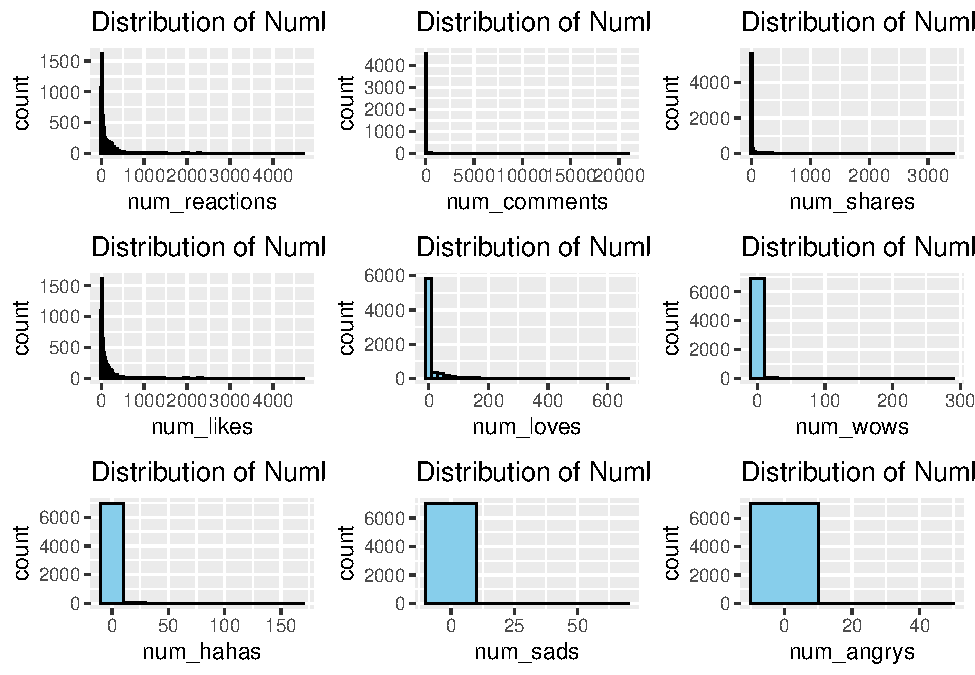
\includegraphics{Final-Report-6303_files/figure-latex/unnamed-chunk-6-1.pdf}

\begin{Shaded}
\begin{Highlighting}[]
\CommentTok{\#Grouped bar plot for comparison between status\_type}
\CommentTok{\# Melt the data frame to long format}
\NormalTok{data\_long }\OtherTok{\textless{}{-}}\NormalTok{ reshape2}\SpecialCharTok{::}\FunctionTok{melt}\NormalTok{(df, }\AttributeTok{id.vars =} \StringTok{"status\_type"}\NormalTok{)}

\CommentTok{\# Create a grouped bar plot}
\FunctionTok{ggplot}\NormalTok{(data\_long, }\FunctionTok{aes}\NormalTok{(}\AttributeTok{x =}\NormalTok{ variable, }\AttributeTok{y =}\NormalTok{ value, }\AttributeTok{fill =}\NormalTok{ status\_type)) }\SpecialCharTok{+}
  \FunctionTok{geom\_bar}\NormalTok{(}\AttributeTok{stat =} \StringTok{"identity"}\NormalTok{, }\AttributeTok{position =} \StringTok{"dodge"}\NormalTok{) }\SpecialCharTok{+}
  \FunctionTok{labs}\NormalTok{(}\AttributeTok{title =} \StringTok{"Comparison of Features for Photo and Video Types"}\NormalTok{,}
       \AttributeTok{x =} \StringTok{"Feature"}\NormalTok{,}
       \AttributeTok{y =} \StringTok{"Value"}\NormalTok{) }\SpecialCharTok{+}
  \FunctionTok{facet\_wrap}\NormalTok{(}\SpecialCharTok{\textasciitilde{}}\NormalTok{ variable, }\AttributeTok{scales =} \StringTok{"free\_y"}\NormalTok{) }\SpecialCharTok{+}
  \FunctionTok{theme\_minimal}\NormalTok{() }\SpecialCharTok{+}
  \FunctionTok{theme}\NormalTok{(}\AttributeTok{axis.text.x =} \FunctionTok{element\_text}\NormalTok{(}\AttributeTok{angle =} \DecValTok{45}\NormalTok{, }\AttributeTok{hjust =} \DecValTok{1}\NormalTok{))}
\end{Highlighting}
\end{Shaded}

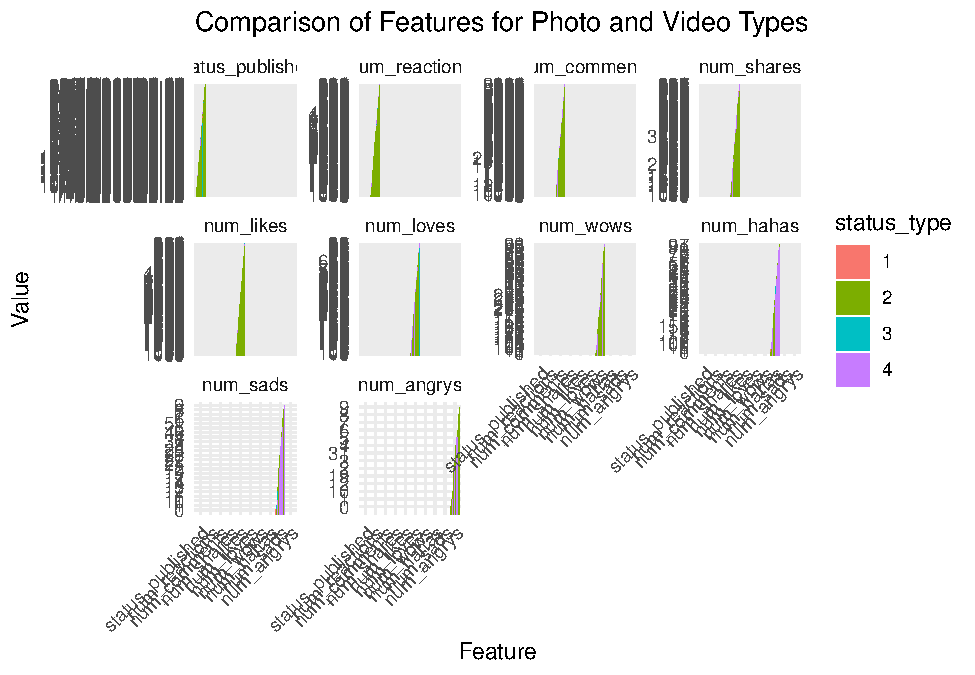
\includegraphics{Final-Report-6303_files/figure-latex/unnamed-chunk-7-1.pdf}

\begin{Shaded}
\begin{Highlighting}[]
\CommentTok{\#Drop status\_published, status\_type}
\NormalTok{data\_subset }\OtherTok{\textless{}{-}} \FunctionTok{select}\NormalTok{(df, }\SpecialCharTok{{-}}\FunctionTok{c}\NormalTok{(}\StringTok{"status\_published"}\NormalTok{,}\StringTok{"status\_type"}\NormalTok{))}

\CommentTok{\#scatterplot matrix}
\FunctionTok{pairs}\NormalTok{(data\_subset)}
\end{Highlighting}
\end{Shaded}

\includegraphics{Final-Report-6303_files/figure-latex/unnamed-chunk-8-1.pdf}

As part of the EDA, we looked at the above plots. A common trend that we
saw is that most reactions tend to amount to 0, i.e, the post didn't
receive said reaction. This makes sense given that it isn't unusual for
a person to provide any more than one like or one comment as part of
interaction with the post.

Looking at the scatterplot matrix, it is clear that num\_reactions has a
highly positive correlation with num\_likes.

\subsubsection{Correlation}\label{correlation}

Having looked at the scatterplot matrix, we plotted the correlation
matrix.

\begin{Shaded}
\begin{Highlighting}[]
\CommentTok{\#calculate correlation matrix}
\NormalTok{correlation\_matrix }\OtherTok{\textless{}{-}} \FunctionTok{cor}\NormalTok{(}\FunctionTok{select}\NormalTok{(df, }\SpecialCharTok{{-}}\FunctionTok{c}\NormalTok{(}\StringTok{"status\_type"}\NormalTok{,}\StringTok{"status\_published"}\NormalTok{)))}

\CommentTok{\#Plot correlation matrix}
\FunctionTok{ggcorrplot}\NormalTok{(correlation\_matrix, }\AttributeTok{type =} \StringTok{"lower"}\NormalTok{, }\AttributeTok{lab =} \ConstantTok{TRUE}\NormalTok{)}
\end{Highlighting}
\end{Shaded}

\includegraphics{Final-Report-6303_files/figure-latex/unnamed-chunk-9-1.pdf}

The correlation only confirmed our findings. num\_reactions has an
almost perfect positive correlation with num\_likes. This indicates that
the increasing number of reactions on the post were directly tied to the
number of likes the post was receiving. The other takeaway here is that
majority of the reactions to the post had to do with liking the post
itself.

\subsection{Modelling and Silhouette}\label{modelling-and-silhouette}

Firstly, we seperate the features with the highest correlations and
scale the the new dataframe.

\begin{Shaded}
\begin{Highlighting}[]
\CommentTok{\#considering num\_likes, num\_reactions, numa\_shares, num\_comments and num\_loves as a datset due to high correlation}
\NormalTok{new\_df }\OtherTok{\textless{}{-}} \FunctionTok{select}\NormalTok{(data\_subset, }\FunctionTok{c}\NormalTok{(}\StringTok{"num\_reactions"}\NormalTok{, }\StringTok{"num\_likes"}\NormalTok{, }\StringTok{"num\_shares"}\NormalTok{,}
                                \StringTok{"num\_comments"}\NormalTok{, }\StringTok{"num\_loves"}\NormalTok{))}
\end{Highlighting}
\end{Shaded}

\begin{Shaded}
\begin{Highlighting}[]
\CommentTok{\#Scaling the Data}
\NormalTok{data\_subset\_scaled }\OtherTok{\textless{}{-}} \FunctionTok{scale}\NormalTok{(new\_df)}
\end{Highlighting}
\end{Shaded}

\subsubsection{K-Means}\label{k-means}

The first step in our modeling was acquiring the optimal amount of
clusters to be used.

\begin{Shaded}
\begin{Highlighting}[]
\CommentTok{\#Modelling}
\CommentTok{\#Kmeans}
\CommentTok{\#Acquiirng the the optimal number of clusters for the model using scree plot}
\FunctionTok{fviz\_nbclust}\NormalTok{(data\_subset\_scaled, kmeans, }\AttributeTok{method=}\StringTok{"wss"}\NormalTok{) }\SpecialCharTok{+}
  \FunctionTok{geom\_vline}\NormalTok{(}\AttributeTok{xintercept =} \DecValTok{4}\NormalTok{, }\AttributeTok{linetype =} \DecValTok{2}\NormalTok{)}
\end{Highlighting}
\end{Shaded}

\includegraphics{Final-Report-6303_files/figure-latex/unnamed-chunk-12-1.pdf}

The plot above shows the optimal number of clusters that should be used
in our model.

\begin{Shaded}
\begin{Highlighting}[]
\CommentTok{\#Kmeans model}
\FunctionTok{set.seed}\NormalTok{(}\DecValTok{7894}\NormalTok{)}
\NormalTok{kmeans\_model }\OtherTok{\textless{}{-}} \FunctionTok{kmeans}\NormalTok{(data\_subset\_scaled, }\AttributeTok{nstart=}\DecValTok{20}\NormalTok{, }\AttributeTok{centers=}\DecValTok{4}\NormalTok{)}
\FunctionTok{print}\NormalTok{(kmeans\_model)}
\end{Highlighting}
\end{Shaded}

\begin{verbatim}
## K-means clustering with 4 clusters of sizes 5932, 373, 117, 628
## 
## Cluster means:
##   num_reactions   num_likes num_shares num_comments  num_loves
## 1    -0.2730390 -0.25552468 -0.2576437   -0.2131312 -0.2516300
## 2     3.4388266  3.56017633 -0.2158710   -0.1834131 -0.2409665
## 3     2.0666203  1.54500160  5.2397437    4.4081884  5.4185703
## 4     0.1515768  0.01124432  1.5856880    1.3008751  1.5104731
## 
## Clustering vector:
##    [1] 4 1 1 1 1 1 4 1 1 1 1 1 1 1 1 1 1 1 1 1 1 1 1 1 1 1 1 1 1 1 1 1 1 1 1 1 1
##   [38] 1 1 1 1 1 1 1 1 1 1 1 1 1 1 1 1 1 1 1 1 1 1 1 1 1 1 1 1 1 1 4 1 1 1 1 1 1
##   [75] 1 1 1 1 1 1 1 1 1 1 1 1 1 1 1 1 1 1 1 1 1 1 1 1 1 3 1 1 1 1 1 1 1 1 1 1 1
##  [112] 1 2 1 1 1 1 1 1 1 1 1 1 1 1 1 1 1 1 1 1 1 1 1 1 1 1 1 1 1 1 1 1 1 1 1 1 1
##  [149] 1 1 1 1 1 1 1 1 1 1 1 1 1 1 1 1 1 1 2 1 1 1 1 1 1 1 1 1 1 1 1 1 1 1 1 1 1
##  [186] 1 1 1 1 1 1 1 1 1 1 1 1 1 4 1 1 1 1 4 1 1 1 1 4 1 1 1 1 1 4 1 1 1 1 1 1 1
##  [223] 1 1 1 4 1 1 1 1 1 1 1 1 1 1 1 1 4 1 1 1 1 1 1 1 1 1 1 1 1 1 1 1 1 1 1 1 1
##  [260] 1 1 1 1 1 1 1 1 1 1 1 1 1 1 1 1 1 1 1 1 1 1 1 1 1 1 1 1 1 1 1 1 1 1 4 1 4
##  [297] 1 1 1 1 1 1 1 1 1 1 1 1 1 1 1 1 1 1 1 1 1 1 1 1 1 1 1 1 1 1 1 1 1 1 1 1 1
##  [334] 1 1 1 1 1 1 1 1 1 1 4 1 1 1 1 1 1 1 1 1 1 1 2 4 1 1 1 1 2 1 1 1 1 1 1 1 1
##  [371] 1 1 1 1 1 1 1 1 1 1 1 1 1 1 1 1 1 1 1 1 1 1 1 1 1 1 1 4 1 1 1 1 1 1 1 1 1
##  [408] 1 1 1 1 1 1 4 1 1 1 1 1 1 1 1 1 1 1 1 1 1 1 1 1 1 1 1 1 1 1 1 1 1 1 1 1 1
##  [445] 1 4 1 1 1 1 1 1 1 1 1 1 1 1 1 1 1 1 1 1 1 1 1 1 1 1 1 1 1 1 1 4 1 1 1 1 3
##  [482] 1 4 1 4 1 4 1 1 1 1 1 1 1 1 1 1 1 3 1 1 1 1 1 1 1 1 1 1 1 1 1 1 1 1 1 1 1
##  [519] 1 1 1 1 1 1 1 1 1 1 1 1 1 1 1 1 1 1 1 1 1 1 1 1 1 1 1 1 1 1 1 1 1 1 1 1 1
##  [556] 1 1 1 1 1 1 1 4 1 1 1 1 1 1 1 1 1 1 1 1 1 1 1 1 1 1 1 1 1 1 1 1 1 1 1 1 1
##  [593] 1 1 1 1 1 1 1 1 1 1 1 1 1 1 1 1 1 1 1 1 1 1 1 1 1 1 1 1 1 1 1 1 1 1 1 1 1
##  [630] 1 1 1 1 1 1 1 1 1 1 1 1 1 1 1 1 1 1 1 1 1 1 1 1 1 1 1 1 1 1 1 1 1 1 1 1 1
##  [667] 1 1 1 1 1 1 1 1 1 1 1 1 1 1 1 1 1 1 1 1 1 1 1 1 1 1 1 1 1 1 1 1 1 1 1 1 1
##  [704] 1 1 1 1 1 1 1 1 1 1 1 1 1 1 1 1 1 1 1 1 1 1 1 3 1 1 1 1 1 1 1 1 1 1 1 1 1
##  [741] 1 1 1 1 1 1 1 1 1 1 1 1 1 1 1 1 1 1 1 1 1 1 1 1 1 1 1 1 1 1 1 1 1 1 1 1 1
##  [778] 1 1 1 1 1 1 1 1 1 1 1 1 1 1 1 1 1 1 1 1 1 1 1 1 1 1 1 1 1 1 1 1 1 1 1 1 1
##  [815] 1 1 1 1 1 1 1 1 1 1 1 1 1 1 1 1 1 1 1 1 1 1 1 1 1 1 1 1 1 1 1 1 1 1 1 1 1
##  [852] 1 1 1 1 1 1 1 1 1 1 1 1 1 1 1 1 1 1 1 1 1 1 1 1 1 1 1 1 1 1 1 1 1 1 1 1 1
##  [889] 1 1 1 1 1 1 1 1 1 1 1 1 1 1 1 1 1 1 1 1 1 1 1 1 1 1 1 1 1 1 1 1 1 1 1 1 1
##  [926] 1 1 1 1 1 1 1 1 1 1 1 1 1 1 1 1 1 1 1 1 1 1 1 1 1 1 1 1 1 1 1 1 1 1 1 1 1
##  [963] 1 1 1 1 1 1 1 1 1 1 1 1 1 1 1 1 1 1 1 1 1 1 1 1 1 1 1 1 1 1 1 1 1 1 1 1 1
## [1000] 1 1 1 1 1 1 1 1 1 1 1 2 1 2 2 2 2 1 2 2 1 2 2 2 1 1 2 1 2 2 2 2 1 2 1 1 2
## [1037] 2 2 2 2 1 2 2 2 2 1 1 2 2 2 1 2 2 1 2 2 2 1 1 1 2 2 2 2 2 2 2 2 2 2 2 2 2
## [1074] 2 2 2 2 2 1 1 1 2 2 2 2 2 2 2 2 2 2 2 2 2 2 2 2 2 2 2 2 2 2 2 2 2 2 2 2 2
## [1111] 2 2 2 2 2 2 2 2 2 2 2 2 2 2 2 2 2 2 2 2 2 2 2 2 2 2 2 2 2 2 2 2 2 2 2 2 2
## [1148] 2 2 2 2 2 2 2 2 2 2 2 1 1 1 2 2 2 2 2 2 2 2 2 2 2 2 2 2 2 2 2 2 2 1 2 2 2
## [1185] 1 2 2 2 2 2 2 2 2 2 2 2 2 2 2 2 2 2 2 2 2 2 2 2 1 1 1 2 2 2 2 2 2 2 2 2 2
## [1222] 2 2 2 2 2 2 2 2 2 2 2 2 2 2 2 2 2 2 2 2 2 2 2 2 2 2 2 2 2 1 2 2 2 2 2 2 2
## [1259] 2 2 2 2 2 2 2 1 2 2 2 2 2 2 2 2 2 2 2 2 2 2 2 2 2 2 2 2 2 2 2 2 2 2 2 2 2
## [1296] 2 2 2 2 2 2 2 2 1 1 2 2 2 2 2 1 2 2 2 1 1 2 1 2 1 1 1 1 1 1 1 1 1 1 2 2 1
## [1333] 2 2 2 2 2 1 1 2 1 2 1 1 2 1 1 1 2 1 2 1 1 1 1 1 1 1 1 1 1 1 1 1 1 1 1 1 1
## [1370] 1 2 1 1 1 1 1 1 1 1 1 1 1 1 1 1 1 1 1 1 1 1 1 1 1 1 1 1 1 1 1 1 1 1 1 2 1
## [1407] 1 1 1 1 1 1 1 2 1 2 1 2 2 2 2 1 1 1 2 1 2 2 1 2 2 2 1 1 1 1 1 2 1 1 1 1 1
## [1444] 1 2 1 2 1 1 1 1 1 1 1 1 1 1 1 1 1 1 1 1 1 1 1 1 1 1 1 1 1 1 1 1 1 1 1 1 1
## [1481] 1 1 1 1 1 1 1 1 1 1 1 1 1 1 1 1 1 1 1 1 2 1 1 1 1 1 1 1 1 1 1 1 1 1 1 1 2
## [1518] 1 1 1 1 1 1 1 1 1 1 1 1 1 1 1 1 1 1 1 1 1 1 1 1 1 1 1 1 1 1 1 1 1 1 1 1 1
## [1555] 1 1 1 1 1 1 1 1 1 1 1 1 1 1 2 1 1 1 1 1 1 1 1 1 1 1 1 1 1 1 1 1 1 1 1 1 1
## [1592] 1 1 1 1 1 1 1 1 1 1 1 1 1 1 1 1 1 1 1 1 1 1 1 1 1 1 1 1 1 1 1 1 1 1 1 1 1
## [1629] 1 1 1 1 1 1 1 1 1 1 1 1 1 1 1 1 1 1 1 1 1 1 1 1 1 1 1 1 1 1 1 1 1 1 1 1 1
## [1666] 1 1 1 1 1 1 1 1 1 1 1 1 1 1 1 1 1 1 1 1 1 2 2 1 1 1 1 1 1 1 1 1 1 1 1 1 1
## [1703] 1 1 1 1 1 1 1 1 1 1 1 1 1 1 1 1 1 1 1 1 1 1 1 1 1 1 1 1 1 1 1 1 1 1 1 1 1
## [1740] 1 1 1 1 1 1 1 1 1 1 1 1 1 1 1 1 1 1 1 1 1 1 1 1 1 1 1 1 1 1 1 1 1 1 1 1 1
## [1777] 1 1 1 1 1 1 1 1 1 1 1 1 1 1 1 1 1 1 1 1 1 1 1 1 1 1 1 1 1 1 1 1 1 1 1 1 1
## [1814] 1 1 1 1 1 1 1 1 1 1 1 1 1 1 1 1 1 1 1 1 1 1 1 1 1 1 1 1 1 1 1 1 1 1 1 1 1
## [1851] 1 1 1 1 1 1 1 1 1 1 1 1 1 1 1 1 1 1 1 1 1 1 1 1 1 1 1 1 1 1 1 1 1 1 1 1 1
## [1888] 1 1 1 1 1 1 1 1 1 1 1 1 1 1 1 1 1 1 1 1 1 1 1 1 1 1 1 1 1 1 1 1 1 1 1 1 1
## [1925] 1 1 1 1 1 1 1 1 1 1 1 1 1 1 1 1 1 1 1 1 1 1 1 1 1 1 1 1 1 1 1 1 1 1 1 1 1
## [1962] 1 1 1 1 1 1 1 1 1 1 1 1 1 1 1 1 1 1 1 1 1 1 1 1 1 1 1 1 1 1 1 1 1 1 1 1 1
## [1999] 1 1 1 1 1 1 1 1 1 1 1 1 1 1 1 1 1 1 1 1 1 1 1 1 1 1 1 1 1 1 1 1 1 1 1 1 1
## [2036] 1 1 1 1 1 1 1 1 1 1 1 1 1 1 1 1 1 1 1 1 1 1 1 1 1 1 1 1 1 1 1 1 1 1 1 1 1
## [2073] 1 1 1 1 1 1 1 1 1 1 1 1 1 1 1 1 1 1 1 1 1 1 1 1 1 1 1 1 1 1 1 1 1 1 1 1 1
## [2110] 1 1 1 1 1 1 1 1 1 1 1 1 1 1 1 1 1 1 1 1 1 1 1 1 1 1 1 1 1 1 1 1 1 1 1 1 1
## [2147] 1 1 1 1 1 1 1 1 1 1 1 1 1 1 1 1 1 1 1 1 1 1 1 1 1 1 1 1 1 1 1 1 1 1 1 1 1
## [2184] 1 1 1 1 1 1 1 1 1 1 1 1 1 1 1 1 1 1 1 1 1 1 1 1 1 1 1 1 1 1 1 1 1 1 1 1 1
## [2221] 1 1 1 1 1 1 1 1 1 1 1 1 1 1 1 1 1 1 1 1 1 1 1 1 1 1 1 1 1 1 1 1 1 1 1 1 1
## [2258] 1 1 1 1 1 1 1 1 1 1 1 1 1 1 1 1 1 1 1 1 1 1 1 1 1 1 1 1 1 1 1 1 1 1 1 1 1
## [2295] 1 1 1 1 1 1 1 1 1 1 1 1 1 1 1 1 1 1 1 1 1 1 1 1 1 1 1 1 1 1 1 1 1 1 1 1 1
## [2332] 1 1 1 1 1 1 1 1 1 1 1 1 1 1 1 1 1 1 1 1 1 1 1 1 1 1 1 1 1 1 1 1 1 1 1 1 1
## [2369] 1 1 1 1 1 1 1 1 1 1 1 1 1 1 1 1 1 1 1 1 1 1 1 1 1 1 1 1 1 1 1 1 1 1 1 1 1
## [2406] 1 1 1 1 1 1 1 1 1 1 1 1 1 1 1 1 1 1 1 1 1 1 1 1 1 1 1 1 1 1 1 1 1 1 1 1 1
## [2443] 1 1 1 1 1 1 1 1 1 1 1 1 1 1 1 1 1 1 1 1 1 1 1 1 1 1 1 1 1 1 1 1 1 1 1 1 1
## [2480] 1 1 1 1 1 1 1 1 1 1 1 1 1 1 1 1 1 1 1 1 1 1 1 1 1 1 1 1 1 1 1 1 1 1 1 1 1
## [2517] 1 1 1 1 1 1 1 1 1 1 1 1 1 1 1 1 1 1 1 1 1 1 1 1 1 1 1 1 1 1 1 1 1 1 1 1 1
## [2554] 1 1 1 1 1 1 1 1 1 1 1 1 1 1 1 1 1 1 1 1 1 1 1 1 1 1 1 1 1 1 1 1 1 1 1 1 1
## [2591] 1 1 1 1 1 1 1 1 1 1 1 1 1 1 1 1 1 1 1 1 1 1 1 1 1 1 1 1 1 1 1 1 1 1 1 1 1
## [2628] 1 1 1 1 1 1 1 1 1 1 4 1 1 1 1 1 1 1 1 1 1 1 1 1 1 1 4 1 1 1 1 1 4 4 1 1 1
## [2665] 1 1 1 1 1 4 1 1 1 1 1 1 4 1 1 1 1 1 1 1 1 1 1 1 1 1 1 1 1 1 1 1 1 1 1 1 1
## [2702] 1 1 1 1 1 1 1 1 1 1 1 1 1 1 1 4 4 1 1 1 1 1 4 1 1 1 1 1 1 4 1 1 1 1 1 1 1
## [2739] 1 1 1 1 1 1 4 1 4 1 1 1 1 1 1 1 1 1 1 1 1 1 1 4 1 1 1 1 1 1 1 1 1 1 1 1 1
## [2776] 1 1 1 1 1 1 1 4 1 1 1 1 1 1 1 1 1 1 1 1 1 4 1 1 1 4 1 1 1 1 1 1 1 1 1 1 1
## [2813] 1 1 1 1 1 1 1 1 1 1 1 1 1 1 1 4 1 1 1 1 1 1 1 1 1 1 1 1 1 1 1 1 4 1 1 1 1
## [2850] 1 1 1 1 1 1 1 1 1 1 4 1 1 4 1 1 1 1 1 1 1 1 1 1 1 1 1 2 1 1 1 1 1 1 1 1 1
## [2887] 1 1 1 1 1 1 1 1 1 1 1 1 1 1 1 4 1 1 1 1 4 1 1 1 1 1 4 1 1 1 1 1 1 3 1 1 1
## [2924] 4 1 1 1 1 1 1 1 1 4 1 1 1 1 1 1 1 1 1 1 1 1 1 1 1 1 1 1 1 1 1 1 1 1 1 1 1
## [2961] 4 1 1 1 1 1 4 1 1 1 1 1 1 1 1 3 2 1 1 1 1 1 4 1 1 1 1 4 1 1 1 1 1 4 1 1 1
## [2998] 1 1 1 4 2 1 1 1 1 1 1 1 1 1 1 1 1 1 1 4 1 1 1 1 1 1 1 1 1 1 1 1 1 1 1 1 1
## [3035] 4 1 1 1 1 1 1 1 1 1 4 1 1 2 1 1 1 1 1 1 1 1 1 1 1 1 1 1 1 1 1 1 1 1 1 1 1
## [3072] 1 1 1 1 1 1 1 2 1 1 1 1 1 4 1 1 1 1 1 1 1 1 4 1 1 1 1 1 1 1 1 1 1 1 1 1 1
## [3109] 1 1 4 1 1 1 1 1 4 1 4 1 1 1 1 1 1 1 1 1 1 1 1 1 1 1 1 1 1 1 1 1 1 1 1 1 1
## [3146] 1 1 1 1 1 1 1 4 1 3 1 1 1 1 1 1 1 1 1 1 1 1 1 1 1 1 1 1 1 1 1 1 1 1 4 1 1
## [3183] 1 1 1 1 1 1 4 1 1 1 1 1 1 4 1 1 4 1 1 1 1 1 1 1 4 1 1 1 4 1 1 1 1 1 1 1 1
## [3220] 1 4 1 1 1 1 1 4 1 4 1 1 1 1 1 1 1 1 1 1 1 1 1 1 1 4 1 3 1 1 1 3 1 1 4 1 1
## [3257] 4 1 1 1 4 1 1 1 1 1 1 1 1 1 1 1 1 1 1 1 1 1 1 1 1 1 1 1 1 1 1 1 1 1 1 1 1
## [3294] 1 1 4 1 3 1 1 4 1 1 1 4 1 1 1 1 1 1 1 1 1 1 1 1 1 1 1 1 1 1 4 1 1 4 1 1 1
## [3331] 1 4 1 1 3 1 1 1 4 1 1 1 1 1 1 1 1 1 4 1 4 4 1 1 1 4 1 1 1 1 1 1 1 1 1 1 1
## [3368] 1 1 1 1 1 1 1 1 1 1 1 1 1 1 1 1 1 1 4 1 1 1 4 1 1 1 1 1 1 1 1 1 4 1 1 1 1
## [3405] 1 1 1 4 1 4 1 1 1 1 1 1 1 1 1 1 1 1 1 1 1 1 1 1 4 1 1 1 1 4 1 1 1 4 1 1 1
## [3442] 1 1 1 1 4 1 1 1 1 1 1 4 1 1 1 1 1 1 1 1 1 1 1 1 1 1 1 1 1 1 1 1 1 1 1 1 1
## [3479] 1 1 1 1 1 1 1 4 1 1 4 1 1 1 1 1 1 1 1 1 4 1 1 4 1 4 1 1 1 1 1 1 1 1 1 4 1
## [3516] 1 1 1 4 1 4 1 1 1 4 1 1 1 1 4 3 1 4 1 1 4 1 1 1 1 1 1 1 4 1 1 1 1 1 1 4 1
## [3553] 1 1 1 1 1 1 1 1 1 1 1 1 1 1 1 1 1 1 1 1 1 1 1 1 1 1 1 1 1 1 1 1 1 1 1 1 1
## [3590] 1 1 1 1 1 1 1 1 1 1 1 1 1 4 1 1 1 4 1 4 1 1 1 1 4 1 4 1 1 1 1 1 1 1 1 1 1
## [3627] 1 1 1 1 1 1 1 1 1 1 1 1 1 1 1 1 1 1 1 1 1 1 1 1 1 1 1 1 1 1 1 1 1 1 1 1 1
## [3664] 1 1 1 1 1 1 1 1 1 1 1 1 1 1 1 1 1 1 1 1 1 1 1 1 1 1 1 1 1 1 1 1 1 1 1 1 1
## [3701] 1 1 1 1 1 1 1 1 1 1 1 1 1 1 1 1 1 1 1 1 1 1 1 1 1 1 1 1 1 1 1 1 1 1 1 1 1
## [3738] 1 1 1 1 1 1 1 1 1 1 1 1 1 1 1 1 1 1 1 1 1 1 1 1 1 1 1 1 1 1 1 1 1 1 1 1 1
## [3775] 1 1 1 1 1 1 1 1 1 1 1 1 1 1 1 1 1 1 1 1 1 1 1 1 1 1 1 1 1 1 1 1 1 1 1 1 1
## [3812] 1 1 1 1 1 1 1 1 1 1 1 1 1 1 1 1 1 1 1 1 1 1 1 1 1 1 1 1 1 1 1 1 1 1 1 1 1
## [3849] 3 1 1 3 1 1 3 1 1 1 3 2 1 1 3 4 3 1 1 3 1 1 3 3 3 4 3 1 3 1 2 1 4 3 3 1 3
## [3886] 3 1 3 1 1 1 3 3 1 4 4 1 3 3 1 1 1 1 1 1 2 1 1 1 1 1 1 1 1 1 1 1 1 1 1 1 1
## [3923] 1 1 1 1 1 1 1 1 1 1 1 1 1 1 1 1 1 1 1 1 1 1 1 1 1 1 1 1 1 1 1 1 1 1 1 1 1
## [3960] 1 1 1 1 1 1 1 1 1 1 1 1 1 1 4 1 1 1 1 1 1 1 4 1 1 1 1 1 4 1 1 4 1 1 1 1 1
## [3997] 1 1 4 1 1 1 1 1 1 1 1 1 1 1 1 1 1 1 1 1 1 1 1 1 1 1 1 1 1 1 1 1 1 1 1 1 1
## [4034] 1 1 1 1 1 1 1 1 1 1 1 1 1 1 1 1 1 1 1 1 1 1 1 1 1 1 1 1 1 1 1 1 1 1 1 1 1
## [4071] 1 1 1 1 1 1 1 1 1 1 1 1 1 1 1 1 1 1 1 1 1 1 1 1 1 1 1 1 1 1 1 1 1 1 1 1 1
## [4108] 1 1 1 1 1 1 1 1 1 1 1 1 1 1 1 1 1 1 1 1 1 1 1 1 1 1 1 1 1 1 1 1 1 1 1 1 1
## [4145] 1 1 1 1 1 1 1 1 4 1 1 1 1 1 1 1 1 1 1 1 1 1 1 1 1 1 1 1 1 1 1 1 1 1 1 1 1
## [4182] 1 1 1 1 1 1 1 1 1 1 1 1 1 1 1 1 1 1 1 1 1 1 1 1 1 1 1 1 1 1 1 1 1 1 1 1 1
## [4219] 1 1 1 1 1 1 1 1 1 1 1 1 1 1 1 1 1 1 1 1 1 1 1 1 1 1 1 1 1 1 1 1 1 1 1 1 1
## [4256] 1 1 1 1 1 1 1 1 1 1 1 1 1 1 1 1 1 1 1 1 1 1 1 1 1 1 1 1 1 1 1 1 1 1 1 1 1
## [4293] 1 1 1 1 1 1 1 1 1 4 1 1 1 1 1 1 1 1 1 1 1 1 1 4 1 1 1 1 1 1 1 1 1 1 4 1 4
## [4330] 1 4 1 1 1 1 1 1 1 1 1 1 1 1 1 1 1 1 1 1 1 1 1 1 1 1 1 1 1 1 1 1 1 1 1 1 1
## [4367] 1 1 1 1 1 1 1 1 1 1 1 1 1 1 1 1 1 1 1 1 1 1 1 1 1 1 1 1 1 1 1 1 1 1 1 1 1
## [4404] 1 1 1 1 1 1 1 1 1 1 1 1 1 1 1 1 1 1 1 1 1 1 1 1 1 1 1 1 1 1 1 1 1 1 1 1 1
## [4441] 1 1 1 1 1 1 1 1 4 1 1 1 1 1 1 1 1 1 1 4 1 1 1 1 1 1 1 1 1 1 1 1 1 1 4 1 1
## [4478] 1 1 2 1 4 4 3 1 4 4 4 3 3 3 3 4 1 4 3 4 2 3 4 1 4 3 4 3 3 3 2 4 3 3 3 2 4
## [4515] 3 4 1 3 3 3 1 4 1 3 3 3 3 3 4 3 3 1 3 3 3 3 1 3 3 1 1 3 3 3 1 1 3 1 3 4 4
## [4552] 4 1 3 1 4 1 3 4 3 1 1 3 1 4 3 1 1 3 1 3 4 1 3 1 4 1 3 1 1 4 1 1 3 1 3 1 4
## [4589] 3 1 3 1 1 1 1 1 1 1 4 1 3 4 1 1 3 3 1 1 3 2 1 3 2 4 1 1 1 1 1 3 1 1 3 1 3
## [4626] 1 1 1 1 1 1 1 1 1 1 1 3 1 1 1 3 1 1 3 2 3 1 4 1 3 1 1 1 1 1 1 1 1 1 1 3 1
## [4663] 2 1 1 1 1 1 2 2 1 2 1 1 1 2 1 1 2 2 2 1 1 2 2 1 1 1 1 1 1 1 1 1 1 1 1 1 1
## [4700] 1 1 1 1 1 1 1 1 1 1 1 1 1 1 1 1 1 1 1 1 1 1 1 1 1 1 1 1 1 1 1 1 1 4 1 1 1
## [4737] 1 1 1 1 1 1 4 1 1 1 1 1 1 1 1 1 4 1 1 1 1 1 1 1 1 1 1 1 1 1 4 1 1 1 1 1 1
## [4774] 1 1 1 4 1 1 1 1 1 1 1 1 1 1 1 1 1 1 1 1 4 1 1 1 1 1 1 1 1 1 4 1 1 1 1 1 1
## [4811] 1 1 4 1 1 1 1 1 1 1 1 1 1 1 4 1 1 1 1 1 1 4 1 1 1 1 1 1 1 1 1 1 4 1 1 1 1
## [4848] 1 1 1 1 1 1 4 1 1 1 1 1 1 1 1 1 1 1 1 1 1 4 1 1 1 1 1 1 1 1 1 1 4 1 1 1 1
## [4885] 4 1 1 1 1 1 1 1 1 1 4 1 1 1 1 1 1 1 1 1 1 1 1 1 1 1 1 1 4 1 1 1 1 1 1 1 1
## [4922] 1 1 4 1 1 1 1 1 1 1 1 1 1 1 1 1 4 1 1 1 1 1 1 1 1 1 4 1 1 1 1 1 1 1 1 1 1
## [4959] 1 1 1 1 1 1 4 1 1 1 1 1 1 1 1 4 1 1 1 1 1 1 1 1 1 1 1 1 1 1 1 1 1 1 1 1 1
## [4996] 1 1 1 1 1 1 4 1 1 1 1 1 1 1 1 1 1 1 1 1 4 1 1 1 1 1 4 1 1 1 1 1 1 1 1 1 1
## [5033] 1 1 1 1 1 1 1 1 1 1 1 1 1 1 1 1 1 1 1 1 4 1 1 1 1 1 1 1 1 1 1 1 1 1 4 1 1
## [5070] 1 1 1 1 1 1 1 1 4 1 1 1 1 1 1 1 1 1 1 1 1 1 1 1 1 1 1 1 1 1 1 1 1 1 1 1 1
## [5107] 1 1 1 1 1 1 1 1 1 1 4 1 1 1 1 1 1 1 1 1 4 1 1 4 1 1 1 1 1 1 1 4 1 1 1 4 1
## [5144] 1 1 1 1 4 1 4 1 1 4 4 1 1 1 4 1 1 1 4 1 1 1 1 4 1 1 4 4 1 4 4 1 1 1 4 1 4
## [5181] 1 4 1 1 4 4 1 1 1 1 1 1 1 4 1 1 4 1 1 4 1 4 4 1 1 4 1 1 4 4 1 4 4 4 4 4 1
## [5218] 1 1 1 1 1 1 4 4 4 4 1 1 1 4 1 1 1 1 1 1 1 4 1 4 1 1 1 1 1 4 1 4 1 1 1 1 1
## [5255] 4 1 1 4 1 1 4 1 4 4 1 4 4 1 1 1 4 1 1 1 4 1 1 1 1 1 1 1 1 4 1 4 4 4 1 4 4
## [5292] 4 4 1 1 1 4 1 1 1 1 4 1 1 4 4 1 1 1 1 4 1 1 4 1 1 1 1 4 1 4 4 1 1 4 1 1 4
## [5329] 1 4 1 4 1 1 4 4 1 4 1 1 1 1 4 1 1 1 4 1 1 1 1 1 1 4 4 4 1 4 4 4 1 4 4 1 4
## [5366] 1 4 1 4 1 1 4 1 4 4 1 1 4 4 4 4 1 4 1 4 4 1 1 4 4 4 1 1 1 1 1 4 1 1 1 1 1
## [5403] 4 1 1 4 1 4 1 4 4 1 1 1 4 4 4 1 1 4 1 1 4 4 1 1 4 1 1 4 1 1 1 4 1 1 4 1 1
## [5440] 4 1 1 1 1 4 1 1 4 1 1 1 1 4 1 4 1 1 1 4 1 1 1 1 1 1 1 1 4 1 1 1 4 1 1 1 1
## [5477] 1 1 1 1 1 4 1 4 4 1 4 1 4 1 1 1 1 4 1 1 4 1 4 4 1 1 4 4 4 1 4 1 4 1 1 4 4
## [5514] 1 1 1 1 4 1 1 4 1 4 1 1 4 1 4 1 4 1 4 4 1 4 4 1 4 4 4 1 4 4 1 4 1 1 1 4 4
## [5551] 1 4 1 1 1 4 1 1 4 1 1 4 4 1 1 4 4 1 4 1 4 4 1 4 1 1 1 4 4 1 4 1 1 4 1 1 4
## [5588] 4 1 4 1 1 4 1 4 1 1 4 1 1 4 1 4 4 1 1 1 4 4 1 1 4 4 1 1 1 4 1 1 1 1 1 1 1
## [5625] 4 1 1 1 1 1 4 1 1 1 1 1 4 1 1 1 1 4 1 1 1 4 1 1 1 1 1 1 4 1 1 1 1 1 1 1 1
## [5662] 1 1 4 1 1 1 1 1 1 4 1 1 1 1 1 1 1 4 1 1 1 1 4 1 1 1 1 1 1 1 4 1 1 4 1 1 1
## [5699] 1 4 1 1 1 1 1 4 1 1 1 4 1 1 1 4 1 1 1 1 1 1 1 1 4 1 1 1 1 4 1 1 4 1 1 4 1
## [5736] 1 1 1 1 1 4 1 1 1 1 4 1 1 1 1 1 1 1 4 1 1 1 1 4 1 1 1 1 4 1 1 1 1 1 1 4 1
## [5773] 1 1 1 1 4 1 1 1 1 1 1 1 4 1 4 1 4 1 1 1 1 1 4 1 1 1 4 1 1 1 4 1 1 1 1 4 1
## [5810] 1 4 1 1 1 4 1 1 1 1 1 4 1 1 4 1 1 4 1 1 1 1 1 4 1 1 1 4 1 1 1 4 1 1 4 1 1
## [5847] 4 1 1 1 4 1 1 1 1 1 4 1 1 1 4 1 4 1 1 4 1 4 1 1 4 1 1 1 1 1 1 1 1 4 1 1 4
## [5884] 1 1 1 1 4 1 1 1 3 1 1 4 1 1 1 1 1 4 1 1 1 4 1 1 4 1 1 1 1 4 1 1 1 4 1 1 4
## [5921] 1 4 1 1 1 1 4 1 1 1 4 1 1 1 1 1 4 1 1 4 1 1 1 1 4 1 1 1 4 1 4 1 1 1 1 4 1
## [5958] 1 1 1 4 1 1 1 1 1 1 4 1 1 1 4 1 1 1 1 4 1 1 1 1 1 4 1 4 4 1 1 1 4 1 1 1 1
## [5995] 1 4 1 1 1 4 4 1 4 1 1 1 4 4 1 1 1 4 1 1 1 4 1 1 4 1 1 1 4 1 1 4 1 1 4 1 1
## [6032] 4 1 1 1 4 1 1 1 4 1 1 1 4 1 1 4 1 4 1 4 1 1 1 1 1 1 4 1 1 4 1 4 1 1 4 1 1
## [6069] 1 4 1 1 1 4 1 4 1 1 1 1 4 1 1 4 1 4 4 1 4 1 4 1 1 4 1 1 4 1 4 1 1 4 1 1 1
## [6106] 1 1 1 1 1 1 1 1 4 1 1 4 1 1 1 1 1 4 1 4 4 1 1 4 1 1 1 4 1 1 1 1 4 1 1 1 1
## [6143] 1 4 1 1 1 1 1 1 4 1 1 4 4 1 4 1 1 1 1 4 1 1 1 1 1 4 4 1 1 1 2 1 1 1 1 1 1
## [6180] 1 1 1 2 1 2 1 1 2 2 2 1 1 2 1 2 1 2 2 2 1 1 1 1 2 1 2 1 1 1 1 2 1 1 1 1 2
## [6217] 1 1 1 2 2 1 1 2 1 1 1 1 1 1 1 1 1 2 1 2 1 1 2 2 2 1 1 2 1 2 1 2 2 2 1 1 1
## [6254] 1 2 1 2 1 1 1 1 2 1 1 1 1 2 1 1 1 2 2 2 4 1 1 4 1 1 4 1 4 4 1 1 1 4 4 4 1
## [6291] 1 3 1 1 1 4 3 2 1 4 4 1 1 4 4 1 1 4 3 1 1 3 4 1 1 1 4 4 1 1 1 4 4 1 1 1 4
## [6328] 4 4 1 1 1 1 1 1 3 1 4 1 1 1 1 4 1 1 1 1 1 1 1 4 1 1 1 1 1 1 1 1 1 1 1 1 1
## [6365] 1 1 1 4 1 4 1 4 1 1 1 1 1 1 1 4 4 1 1 1 1 4 4 1 4 1 1 1 4 1 1 1 1 4 4 1 1
## [6402] 1 3 1 4 1 1 1 1 1 1 4 1 1 4 1 1 4 1 1 1 1 1 1 1 1 4 1 1 4 1 1 1 4 1 1 1 1
## [6439] 1 1 1 1 1 1 1 1 1 1 3 1 1 1 1 1 1 1 1 1 1 1 1 1 1 1 1 1 1 1 1 1 1 1 1 1 1
## [6476] 1 1 1 1 1 1 1 1 1 1 1 1 1 1 1 1 1 1 1 1 1 1 1 1 1 1 1 1 1 1 4 1 1 1 1 1 1
## [6513] 1 1 1 1 1 1 1 1 1 1 1 4 1 1 1 1 1 1 1 1 1 1 1 1 1 1 1 1 1 1 1 1 1 1 1 1 1
## [6550] 1 1 4 1 1 1 1 1 1 1 4 1 4 1 1 1 1 4 1 1 1 1 1 1 4 1 1 1 1 1 1 1 1 1 1 1 1
## [6587] 1 1 1 1 1 1 1 1 1 1 1 1 1 1 1 1 1 1 1 1 1 1 1 1 4 1 1 1 1 4 4 1 1 1 1 1 1
## [6624] 1 4 4 1 1 1 1 1 1 1 1 1 4 1 1 4 1 1 3 1 1 1 1 1 1 4 1 1 1 1 1 1 1 1 1 1 4
## [6661] 1 1 1 1 1 1 1 1 1 1 1 1 1 1 1 1 1 1 1 1 1 1 1 1 1 1 1 1 1 1 1 1 1 1 1 1 1
## [6698] 1 1 1 1 3 1 1 1 4 4 1 1 1 1 1 1 1 1 4 1 4 1 1 1 1 4 1 1 1 1 4 1 4 1 1 1 1
## [6735] 1 4 4 3 1 4 1 1 1 1 1 4 1 1 1 4 1 1 4 1 4 1 1 3 1 1 1 1 3 1 4 1 1 4 1 4 4
## [6772] 1 1 1 1 3 1 1 1 1 1 1 1 1 1 4 4 3 1 1 1 1 1 1 1 1 3 1 1 3 4 1 1 1 1 1 1 1
## [6809] 3 1 3 1 1 1 3 1 1 1 1 4 1 1 4 1 1 1 1 3 1 1 1 1 1 1 4 4 1 4 1 4 1 1 1 4 4
## [6846] 1 1 1 4 1 1 4 1 4 1 1 1 1 1 1 1 4 1 1 1 4 1 1 1 4 1 1 1 4 1 1 1 1 1 1 1 1
## [6883] 1 1 1 1 1 1 1 1 1 1 4 1 4 1 1 1 1 1 1 1 1 1 1 1 4 4 1 1 4 1 4 1 1 4 1 1 1
## [6920] 4 1 1 4 1 1 1 1 4 1 1 1 1 4 1 1 4 1 4 1 4 1 1 1 1 4 1 1 1 1 4 1 1 1 1 1 4
## [6957] 1 1 1 4 1 1 4 1 4 1 1 1 1 1 1 1 1 1 4 1 1 4 4 1 1 1 1 1 1 1 1 1 1 1 1 1 1
## [6994] 1 1 1 1 1 1 1 1 2 1 1 1 1 1 1 1 1 1 1 1 1 1 1 1 1 1 1 1 1 1 1 1 1 1 1 1 1
## [7031] 1 1 1 1 1 1 1 1 1 1 1 1 1 1 1 1 1 1 1 1
## 
## Within cluster sum of squares by cluster:
## [1] 1813.184 1570.676 4334.677 2678.759
##  (between_SS / total_SS =  70.5 %)
## 
## Available components:
## 
## [1] "cluster"      "centers"      "totss"        "withinss"     "tot.withinss"
## [6] "betweenss"    "size"         "iter"         "ifault"
\end{verbatim}

\begin{Shaded}
\begin{Highlighting}[]
\NormalTok{data\_subset}\SpecialCharTok{$}\NormalTok{cluster }\OtherTok{\textless{}{-}}\NormalTok{ kmeans\_model}\SpecialCharTok{$}\NormalTok{cluster}

\FunctionTok{pairs}\NormalTok{(data\_subset[, }\SpecialCharTok{{-}}\FunctionTok{ncol}\NormalTok{(data\_subset)], }
      \AttributeTok{col =}\NormalTok{ kmeans\_model}\SpecialCharTok{$}\NormalTok{cluster, }
      \AttributeTok{pch =} \DecValTok{16}\NormalTok{, }
      \AttributeTok{main =} \StringTok{"Scatterplot Matrix with Clusters"}\NormalTok{)}
\end{Highlighting}
\end{Shaded}

\includegraphics{Final-Report-6303_files/figure-latex/unnamed-chunk-14-1.pdf}

Above is a scatter plot matrix of all the interactions with the posts
color coded by the clusters within which they are present.

\begin{Shaded}
\begin{Highlighting}[]
\CommentTok{\#Aggregating the clusters}
\FunctionTok{kable}\NormalTok{(}\FunctionTok{aggregate}\NormalTok{(data\_subset\_scaled, }\AttributeTok{by=}\FunctionTok{list}\NormalTok{(}\AttributeTok{cluster=}\NormalTok{kmeans\_model}\SpecialCharTok{$}\NormalTok{cluster), mean),}
      \AttributeTok{format =} \StringTok{"latex"}\NormalTok{,}
      \AttributeTok{booktabs =} \ConstantTok{TRUE}\NormalTok{) }\SpecialCharTok{\%\textgreater{}\%} \FunctionTok{kable\_styling}\NormalTok{(}\AttributeTok{position=}\StringTok{"center"}\NormalTok{)}
\end{Highlighting}
\end{Shaded}

\begin{table}
\centering
\begin{tabular}{rrrrrr}
\toprule
cluster & num\_reactions & num\_likes & num\_shares & num\_comments & num\_loves\\
\midrule
1 & -0.2730390 & -0.2555247 & -0.2576437 & -0.2131312 & -0.2516300\\
2 & 3.4388266 & 3.5601763 & -0.2158710 & -0.1834131 & -0.2409665\\
3 & 2.0666203 & 1.5450016 & 5.2397437 & 4.4081884 & 5.4185703\\
4 & 0.1515768 & 0.0112443 & 1.5856880 & 1.3008751 & 1.5104731\\
\bottomrule
\end{tabular}
\end{table}

This is another visualization for the scatterplot matrix from earlier
that shows the clustering more clearly.

\begin{Shaded}
\begin{Highlighting}[]
\CommentTok{\#cluster visualization}
\FunctionTok{fviz\_cluster}\NormalTok{(kmeans\_model, data\_subset)}
\end{Highlighting}
\end{Shaded}

\includegraphics{Final-Report-6303_files/figure-latex/unnamed-chunk-16-1.pdf}

\begin{Shaded}
\begin{Highlighting}[]
\CommentTok{\# Calculate silhouette scores}
\NormalTok{silhouette\_scores }\OtherTok{\textless{}{-}} \FunctionTok{silhouette}\NormalTok{(kmeans\_model}\SpecialCharTok{$}\NormalTok{cluster, }\FunctionTok{dist}\NormalTok{(data\_subset\_scaled))}

\CommentTok{\# Mean silhouette score}
\NormalTok{mean\_silhouette\_score }\OtherTok{\textless{}{-}} \FunctionTok{mean}\NormalTok{(silhouette\_scores[, }\StringTok{"sil\_width"}\NormalTok{])}
\FunctionTok{print}\NormalTok{(mean\_silhouette\_score)}
\end{Highlighting}
\end{Shaded}

\begin{verbatim}
## [1] 0.7568841
\end{verbatim}

Our K-means model received a silhouette score of \textbf{0.7578}.

This suggests that the clusters are well-separated and that each data
point is relatively close to its own cluster centroid compared to other
clusters. This indicates a strong clustering structure in our data,
where the clusters are distinct and well-defined.

\subsubsection{K-Medioids}\label{k-medioids}

Much like K-Means, we derive the optimal number of clusters for the
K-Medioids model

\begin{Shaded}
\begin{Highlighting}[]
\CommentTok{\#Kmedioids}
\FunctionTok{fviz\_nbclust}\NormalTok{(data\_subset\_scaled, pam, }\AttributeTok{method=}\StringTok{"wss"}\NormalTok{) }\SpecialCharTok{+}
  \FunctionTok{geom\_vline}\NormalTok{(}\AttributeTok{xintercept =} \DecValTok{5}\NormalTok{, }\AttributeTok{linetype =} \DecValTok{2}\NormalTok{)}
\end{Highlighting}
\end{Shaded}

\includegraphics{Final-Report-6303_files/figure-latex/unnamed-chunk-18-1.pdf}

\begin{Shaded}
\begin{Highlighting}[]
\FunctionTok{set.seed}\NormalTok{(}\DecValTok{7894}\NormalTok{)}
\NormalTok{kmed\_model }\OtherTok{\textless{}{-}} \FunctionTok{pam}\NormalTok{(data\_subset\_scaled, }\AttributeTok{k=}\DecValTok{5}\NormalTok{)}
\FunctionTok{print}\NormalTok{(kmed\_model)}
\end{Highlighting}
\end{Shaded}

\begin{verbatim}
## Medoids:
##        ID num_reactions  num_likes num_shares num_comments  num_loves
## [1,] 5423  -0.000253257 -0.1269113  1.3296162    0.7662048  1.3076686
## [2,] 2220  -0.447699594 -0.4272635 -0.3041228   -0.2488162 -0.3184318
## [3,] 3925   0.176996017  0.1956892 -0.2585301   -0.2105983 -0.1933472
## [4,] 3872   1.307500530  0.8698130  4.8934469    4.1529801  5.1102420
## [5,] 1272   3.646326311  3.7865663 -0.2433325   -0.1869932 -0.3184318
## Clustering vector:
##    [1] 1 2 3 2 3 3 1 3 3 3 3 3 3 3 3 3 2 2 3 2 3 3 2 2 2 2 2 2 2 3 2 2 2 2 2 3 2
##   [38] 2 2 3 2 2 3 3 3 3 3 2 3 3 2 2 2 1 3 3 3 2 2 3 3 3 3 3 2 2 3 1 3 3 2 3 3 2
##   [75] 3 2 3 2 3 2 2 2 2 3 3 2 3 3 3 2 2 2 3 3 3 2 3 3 3 4 2 2 2 2 2 2 2 3 3 3 3
##  [112] 3 3 3 3 3 3 3 3 3 3 3 2 2 3 3 2 3 3 3 3 2 2 2 2 2 2 2 2 2 3 2 3 3 3 2 3 2
##  [149] 2 3 3 3 3 3 3 3 2 2 2 3 2 2 2 2 3 3 5 3 3 3 2 2 2 3 3 2 2 3 2 2 2 3 2 2 2
##  [186] 2 2 3 3 2 3 2 2 2 3 2 3 3 1 2 2 2 2 1 2 3 2 2 1 2 2 2 2 2 1 2 2 3 3 3 3 3
##  [223] 3 3 3 1 3 2 3 3 2 2 3 3 3 3 3 2 1 3 3 3 3 3 2 3 3 3 3 3 3 3 2 3 3 3 3 3 3
##  [260] 3 2 3 3 2 3 2 3 2 2 2 2 3 2 2 2 2 2 3 3 2 3 3 3 3 2 2 2 3 3 3 2 2 3 1 3 1
##  [297] 3 3 3 3 2 3 3 2 3 3 2 3 3 3 3 3 3 3 2 2 2 3 3 2 2 2 2 2 3 2 3 2 3 3 3 2 2
##  [334] 2 2 3 3 3 3 2 2 2 3 1 3 2 3 3 3 3 3 3 3 3 3 5 1 3 2 2 3 3 3 2 3 2 2 3 2 2
##  [371] 2 3 2 3 3 3 1 2 3 3 2 2 3 2 2 3 2 2 2 2 2 2 2 2 3 3 2 1 3 3 3 3 3 3 3 3 3
##  [408] 3 3 3 3 2 2 1 2 2 3 3 3 3 2 3 3 3 3 2 3 3 3 3 2 2 3 3 3 3 3 3 3 3 2 3 2 3
##  [445] 3 1 3 3 3 3 2 2 2 3 3 3 2 3 3 2 3 3 3 2 3 2 3 2 3 2 3 3 3 3 3 1 2 3 3 3 4
##  [482] 2 4 3 1 3 1 3 3 2 2 3 3 2 3 3 2 3 4 3 3 2 2 3 2 2 2 3 2 2 3 2 2 2 3 2 2 2
##  [519] 3 2 3 3 2 2 3 3 2 2 3 3 3 3 3 2 2 2 3 3 2 2 2 3 2 2 3 3 3 2 2 2 2 2 3 2 2
##  [556] 2 3 2 3 3 3 2 1 2 3 2 2 2 3 2 2 3 2 3 2 2 2 2 2 2 3 2 3 3 2 2 3 3 2 3 2 2
##  [593] 2 2 2 2 2 2 2 2 3 3 2 3 2 2 2 3 2 2 3 2 2 2 2 2 2 3 2 2 2 3 2 2 2 2 2 2 2
##  [630] 3 3 3 2 3 3 3 3 3 3 2 2 3 2 3 2 3 3 3 2 2 2 2 3 2 3 3 3 2 2 3 2 3 3 2 2 3
##  [667] 3 2 2 2 2 2 2 2 2 2 2 3 3 3 2 2 2 2 3 2 2 2 2 2 3 3 3 2 3 3 2 3 3 2 2 3 2
##  [704] 3 2 3 3 3 2 2 3 3 3 2 3 2 3 3 2 2 2 2 2 2 2 3 4 2 2 2 3 2 2 2 2 2 2 2 2 2
##  [741] 2 2 2 2 3 2 3 2 3 2 2 2 3 3 3 2 2 3 2 3 2 2 2 2 2 3 3 2 2 2 3 2 3 3 3 2 2
##  [778] 3 3 3 2 3 3 2 3 3 2 3 2 3 2 2 2 2 2 2 2 2 2 2 2 2 3 3 3 3 2 2 2 2 3 3 2 2
##  [815] 2 3 3 3 2 2 3 2 3 3 2 2 3 2 3 3 2 3 2 2 2 2 2 3 3 3 3 2 2 2 3 2 2 3 3 2 2
##  [852] 2 3 2 2 2 2 2 3 2 2 3 3 2 3 2 2 3 3 3 2 2 3 2 2 2 2 2 2 3 2 2 2 2 2 2 2 2
##  [889] 3 2 3 3 3 2 3 2 2 2 2 2 2 2 2 3 2 2 3 3 2 2 3 2 3 3 2 3 2 2 2 2 2 2 2 2 2
##  [926] 2 2 2 2 3 3 2 3 3 3 2 3 3 3 3 3 3 3 3 3 3 3 3 3 3 3 2 3 3 2 2 3 3 3 3 3 2
##  [963] 2 2 2 3 2 3 3 3 3 2 3 2 2 2 3 3 2 2 2 2 3 3 2 3 3 2 2 3 3 3 2 2 2 2 2 2 2
## [1000] 3 2 2 2 2 3 2 2 2 2 2 3 3 5 5 5 3 3 3 5 3 5 3 5 2 2 5 3 5 5 3 5 3 5 3 3 3
## [1037] 5 3 3 3 3 5 5 3 5 3 2 5 5 5 3 5 5 3 3 3 5 3 3 3 5 5 5 5 5 5 5 5 5 5 5 5 5
## [1074] 5 5 5 3 5 3 2 3 5 5 3 5 5 5 5 5 5 3 3 5 5 3 5 5 3 5 3 5 5 5 5 5 5 5 5 5 5
## [1111] 5 5 5 5 5 5 5 3 5 5 5 5 5 5 5 5 5 5 5 5 5 5 5 5 5 5 5 5 5 5 5 5 5 5 5 5 5
## [1148] 5 5 5 5 5 5 5 5 5 5 5 2 2 2 5 5 5 5 5 5 5 5 5 5 5 5 5 5 5 5 5 5 5 2 5 5 5
## [1185] 2 5 5 5 5 5 5 5 5 5 5 5 5 5 5 5 5 5 5 5 5 5 5 5 3 3 3 5 5 5 5 5 5 5 5 5 5
## [1222] 5 5 5 5 5 5 5 5 5 5 5 5 5 5 5 5 5 5 5 5 5 5 5 5 5 5 5 5 5 3 5 5 5 3 5 5 3
## [1259] 5 5 5 5 5 3 5 3 5 5 5 5 5 5 5 5 5 5 5 5 5 5 5 5 5 5 5 5 5 5 5 5 5 5 5 5 5
## [1296] 5 5 5 5 5 5 5 5 2 3 5 5 5 5 5 3 5 5 5 2 2 3 3 3 3 3 2 2 2 2 2 2 2 3 5 5 3
## [1333] 3 5 5 5 5 3 3 5 2 5 3 3 5 3 3 3 3 3 5 3 3 3 3 3 3 3 3 3 3 3 3 3 3 3 3 3 3
## [1370] 3 3 3 2 3 3 3 3 3 3 3 2 3 3 3 3 2 3 2 3 3 3 3 3 3 3 3 3 3 3 3 3 2 3 3 5 3
## [1407] 3 3 3 3 3 3 3 5 3 3 3 5 5 5 5 3 3 3 5 3 5 5 3 5 5 5 3 3 3 2 3 5 3 2 3 3 3
## [1444] 3 5 3 3 3 3 3 3 3 3 3 3 3 3 3 3 3 3 3 3 3 3 3 2 3 3 3 2 3 3 3 3 3 3 3 3 3
## [1481] 2 3 2 2 3 3 3 3 3 3 3 3 3 3 2 3 3 3 3 3 3 3 3 3 3 3 3 3 3 3 3 3 3 3 3 3 3
## [1518] 3 3 3 3 3 3 3 3 3 3 3 3 2 3 3 3 3 2 3 3 2 3 2 2 3 3 3 3 3 2 2 3 2 2 2 2 3
## [1555] 2 3 2 2 2 2 2 2 3 3 2 2 2 2 5 2 2 2 3 3 3 2 2 3 2 3 3 2 2 3 3 3 3 3 2 2 2
## [1592] 3 2 2 2 3 2 2 3 2 2 2 2 3 2 2 2 2 3 2 2 2 2 3 3 2 3 2 3 3 3 3 2 3 3 3 2 2
## [1629] 3 2 2 2 2 3 3 3 2 2 3 3 3 3 3 2 2 3 3 2 2 3 3 2 2 2 2 2 2 2 2 2 2 3 2 2 3
## [1666] 2 3 2 3 2 2 2 2 2 2 3 2 2 2 2 2 2 2 2 2 2 5 5 2 2 2 2 3 2 2 2 3 2 3 2 3 2
## [1703] 2 3 2 3 2 3 2 2 2 2 2 2 2 2 2 2 2 2 2 2 2 2 2 2 2 2 2 3 2 2 2 2 2 2 2 2 2
## [1740] 2 2 2 2 2 2 2 2 2 2 2 2 2 2 2 2 2 2 2 2 2 2 2 2 2 2 2 2 2 2 2 2 2 2 2 2 2
## [1777] 2 2 2 2 2 2 2 2 2 2 2 2 2 2 2 2 2 2 2 2 2 2 2 2 2 2 2 2 2 2 2 2 2 2 2 2 2
## [1814] 2 2 2 2 2 2 2 2 2 2 2 2 2 2 2 2 2 2 2 2 2 2 2 2 2 2 2 2 2 2 2 2 2 2 2 2 2
## [1851] 2 2 2 2 2 2 2 2 2 2 2 2 2 2 2 2 2 2 2 2 2 2 2 2 2 2 2 2 2 2 3 2 2 2 2 2 2
## [1888] 2 2 2 2 2 2 2 2 2 2 2 2 2 2 2 2 2 2 2 2 2 2 2 2 2 2 2 2 2 2 2 2 2 2 2 2 2
## [1925] 2 2 2 2 2 2 2 2 2 2 2 2 2 2 2 2 2 2 2 2 2 2 2 2 2 2 2 2 2 2 2 2 2 2 2 2 2
## [1962] 2 2 2 2 2 2 2 2 2 2 2 2 2 2 2 2 2 2 2 2 2 2 2 2 2 2 2 2 2 2 2 2 2 2 2 2 2
## [1999] 2 2 2 2 2 2 2 2 2 2 2 2 2 2 2 2 2 2 2 2 2 2 2 2 2 2 2 2 2 2 2 2 2 2 2 2 2
## [2036] 2 2 2 2 2 2 2 2 2 2 2 2 2 2 2 2 2 2 2 2 2 2 2 2 2 2 2 2 2 2 2 2 2 2 2 2 2
## [2073] 2 2 2 2 2 2 2 2 2 2 2 2 2 2 2 2 2 2 2 2 2 2 2 2 2 2 2 2 2 2 2 2 2 2 2 2 2
## [2110] 2 2 2 2 2 2 2 2 2 2 2 2 2 2 2 2 2 2 2 2 2 2 2 2 2 2 2 2 2 2 2 2 2 2 2 2 2
## [2147] 2 2 2 2 2 2 2 2 2 2 2 2 2 2 2 2 2 2 2 2 2 2 2 2 2 2 2 2 2 2 2 2 2 2 2 2 2
## [2184] 2 2 2 2 2 2 2 2 2 2 2 2 2 2 2 2 2 2 2 2 2 2 2 2 2 2 2 2 2 2 2 2 2 2 2 2 2
## [2221] 2 2 2 2 2 2 2 2 2 2 2 2 2 2 2 2 2 2 2 2 2 2 2 2 2 2 2 2 2 2 2 2 2 2 2 2 2
## [2258] 2 2 2 2 2 2 2 2 2 2 2 2 2 2 2 2 2 2 2 2 2 2 2 2 2 2 2 2 2 2 2 2 2 2 2 2 2
## [2295] 2 2 2 2 2 2 2 2 2 2 2 2 2 2 2 2 2 2 2 2 2 2 2 2 2 2 2 2 2 2 2 2 2 2 2 2 2
## [2332] 2 2 2 2 2 2 2 2 2 2 2 2 2 2 2 2 2 2 2 2 2 2 2 2 2 2 2 2 2 2 2 2 2 2 2 2 2
## [2369] 2 2 2 2 2 2 2 2 2 2 2 2 2 2 2 2 2 2 2 2 2 2 2 2 2 2 2 2 2 2 2 2 2 2 2 2 2
## [2406] 2 2 2 2 2 2 2 2 2 2 2 2 2 2 2 2 2 2 2 2 2 2 2 2 2 2 2 2 2 2 2 2 2 2 2 2 2
## [2443] 2 2 2 2 2 2 2 2 2 2 2 2 2 2 2 2 2 2 2 2 2 2 2 2 2 2 2 2 2 2 2 2 2 2 2 2 2
## [2480] 2 2 2 2 2 2 2 2 2 2 2 2 2 2 2 2 2 2 2 2 2 2 2 2 2 2 2 2 2 2 2 2 2 2 2 2 2
## [2517] 2 2 2 2 2 2 2 2 2 2 2 2 2 2 2 2 2 2 2 2 2 2 2 2 2 2 2 2 2 2 2 2 2 2 2 2 2
## [2554] 2 2 2 2 2 2 2 2 2 2 2 2 2 2 2 2 2 2 2 2 2 2 2 2 2 2 2 2 2 2 2 2 2 2 2 2 2
## [2591] 2 2 2 2 2 2 2 2 2 2 2 2 2 2 2 2 2 2 2 2 2 2 2 2 2 2 2 2 2 2 2 2 2 2 2 2 2
## [2628] 2 2 2 2 2 2 2 2 2 2 1 2 2 2 2 2 1 2 3 2 2 2 2 2 2 2 1 2 2 2 2 2 1 1 2 2 2
## [2665] 3 2 2 2 2 1 3 2 2 2 2 2 1 3 2 2 2 2 2 2 2 2 2 2 3 2 2 2 2 2 2 2 2 2 2 2 2
## [2702] 2 2 2 2 2 2 2 2 2 2 2 2 2 2 2 1 1 2 2 2 2 2 1 2 2 2 3 2 2 1 2 3 2 2 2 2 2
## [2739] 3 2 2 2 2 2 1 2 1 2 2 2 2 2 2 2 2 2 2 2 2 2 2 1 2 2 2 2 2 2 2 2 2 2 2 2 2
## [2776] 2 2 2 2 2 2 2 1 2 2 2 3 2 2 2 2 2 2 2 2 2 1 2 2 2 1 2 2 2 2 2 2 2 2 2 2 2
## [2813] 2 2 2 2 2 2 2 2 2 2 2 2 2 1 2 1 2 2 3 2 2 2 2 1 2 2 2 2 2 3 2 2 1 2 2 2 2
## [2850] 2 2 2 2 3 2 2 2 2 2 1 2 2 1 2 2 2 2 2 2 2 2 3 2 2 3 2 5 2 2 2 3 3 2 2 2 2
## [2887] 2 2 2 2 2 2 3 2 2 2 2 2 3 2 2 1 2 2 3 2 1 2 2 2 2 2 1 3 2 2 2 2 2 4 2 2 2
## [2924] 1 2 2 2 2 2 2 2 2 1 3 2 2 2 2 2 2 2 2 2 2 2 2 2 2 2 2 2 2 2 2 2 2 2 2 2 2
## [2961] 1 2 2 2 2 2 1 2 2 2 2 3 2 2 2 4 3 2 2 2 3 2 1 2 2 2 2 1 2 2 2 2 2 1 2 2 2
## [2998] 2 2 2 1 5 2 2 2 2 2 2 2 2 2 2 2 2 2 2 1 2 2 2 2 2 2 2 2 2 2 3 3 2 2 2 2 2
## [3035] 1 2 2 2 3 2 2 2 2 3 1 3 2 5 2 2 3 2 2 2 2 2 2 2 2 2 3 2 2 2 2 2 2 2 2 2 2
## [3072] 2 2 3 3 2 2 2 5 2 2 2 3 2 1 2 3 2 2 3 3 2 2 1 3 2 2 2 2 2 3 2 2 2 2 3 3 3
## [3109] 3 2 1 2 2 2 2 2 1 2 1 2 2 2 3 2 2 2 2 2 2 2 3 2 2 2 3 2 2 2 3 2 3 2 2 2 2
## [3146] 2 3 2 2 2 3 2 1 2 4 2 3 2 3 2 2 3 2 2 3 3 2 2 3 3 3 2 2 2 2 1 1 2 2 1 2 2
## [3183] 3 3 2 2 2 2 1 2 2 2 2 2 2 1 2 2 1 2 2 2 2 1 2 2 1 2 2 2 1 2 2 2 3 2 2 2 3
## [3220] 2 1 3 2 2 3 2 1 2 1 2 2 2 3 2 2 1 2 2 2 2 2 1 2 2 1 2 4 2 2 2 4 3 2 1 2 2
## [3257] 1 2 2 2 1 2 2 2 3 2 2 2 2 2 2 2 2 2 2 2 2 2 2 2 2 2 2 2 2 2 3 2 2 2 2 3 2
## [3294] 3 2 1 2 4 2 2 1 2 2 2 4 3 2 2 2 2 2 2 2 3 2 2 2 2 2 2 2 2 2 1 2 2 1 2 3 2
## [3331] 2 1 3 2 4 2 2 2 1 2 2 2 2 2 2 2 2 2 1 2 1 1 2 2 2 4 3 2 1 2 2 2 2 2 2 2 2
## [3368] 2 2 3 2 2 2 3 2 2 2 2 2 2 2 2 3 3 2 1 2 2 2 1 2 3 1 2 2 2 2 2 2 1 2 2 3 2
## [3405] 3 2 2 1 2 1 2 2 2 2 2 2 2 2 2 2 2 2 2 2 2 2 3 2 1 2 2 2 2 1 2 2 2 1 2 3 2
## [3442] 2 3 2 2 1 2 2 2 2 2 2 1 2 2 2 2 2 2 2 2 2 1 3 2 2 2 2 2 2 3 2 2 3 3 2 2 2
## [3479] 3 2 2 2 2 3 2 1 3 3 1 2 2 2 2 2 2 2 2 3 1 2 2 1 2 1 2 2 3 2 3 2 2 2 3 1 3
## [3516] 3 2 2 1 2 1 2 3 2 1 2 3 2 2 1 4 2 1 3 2 1 2 2 3 1 2 2 2 1 2 2 2 2 2 2 1 3
## [3553] 2 3 2 3 2 2 3 2 2 3 2 2 2 2 3 3 3 2 2 2 2 2 2 2 2 2 3 3 2 2 2 2 2 2 2 2 3
## [3590] 1 2 2 2 2 2 3 3 2 1 2 2 2 1 2 2 2 1 2 1 2 2 2 2 1 3 1 2 2 2 2 2 2 2 2 2 2
## [3627] 2 2 2 2 2 2 2 2 2 3 3 2 2 2 2 2 2 2 2 2 2 2 2 2 2 2 2 2 2 2 2 2 2 2 2 2 2
## [3664] 2 2 2 2 2 2 2 2 2 2 2 2 2 2 2 2 2 2 2 2 2 2 2 2 2 2 2 2 2 2 2 2 2 2 2 2 2
## [3701] 2 2 2 2 2 2 2 2 2 2 2 2 2 2 2 2 2 2 3 2 2 2 2 2 2 2 2 2 2 2 2 2 2 2 2 2 2
## [3738] 2 2 2 2 2 2 2 2 2 2 3 2 2 2 2 2 2 2 2 2 2 2 2 2 2 2 2 2 2 2 2 2 2 2 2 2 2
## [3775] 2 2 2 2 2 2 2 2 2 2 2 2 2 2 2 2 2 2 2 2 2 2 2 2 2 2 2 2 2 2 2 2 2 2 2 2 2
## [3812] 2 2 2 2 2 2 2 2 2 2 2 2 2 2 2 2 2 2 2 2 2 2 2 2 2 2 2 2 2 2 2 2 2 2 2 2 3
## [3849] 4 3 3 4 3 3 4 3 3 3 4 5 3 3 4 1 4 3 3 4 3 3 4 4 4 1 4 3 4 3 5 3 1 4 4 3 4
## [3886] 4 3 4 3 3 1 4 4 3 1 1 3 4 4 3 3 3 3 3 3 5 3 3 3 3 3 3 3 3 3 2 2 3 2 3 3 2
## [3923] 3 3 3 3 3 3 3 3 3 3 3 3 3 3 3 3 2 3 3 3 3 2 2 2 3 2 2 2 3 2 2 2 3 2 2 3 2
## [3960] 2 2 3 2 3 2 2 2 2 3 2 2 2 3 1 2 2 2 2 3 2 2 1 2 2 1 3 2 1 2 3 1 2 2 3 3 3
## [3997] 3 2 1 2 2 3 2 2 1 2 2 2 3 2 3 2 2 2 2 2 2 2 2 2 2 3 2 2 2 2 2 2 2 2 2 2 2
## [4034] 2 2 2 2 2 2 2 2 2 2 2 2 2 2 2 2 2 2 2 2 2 2 2 2 2 2 2 2 2 2 2 2 2 2 2 2 2
## [4071] 2 2 2 2 2 2 2 2 2 2 2 2 2 2 2 2 2 2 2 2 2 2 2 2 2 2 2 2 2 2 2 2 2 2 2 2 2
## [4108] 2 2 2 2 2 2 2 2 2 2 2 2 2 2 2 2 2 2 2 2 2 2 2 2 2 2 2 2 2 2 2 2 2 2 2 2 2
## [4145] 2 2 2 2 2 2 2 2 1 2 2 2 2 2 2 2 2 2 2 2 2 2 2 2 2 2 2 2 2 2 2 2 2 2 2 2 2
## [4182] 2 2 2 2 2 2 2 2 2 2 2 2 2 2 2 2 2 2 2 2 2 2 2 2 2 2 2 2 2 2 2 2 2 2 2 2 2
## [4219] 2 2 2 2 2 2 2 2 2 2 2 2 2 2 2 2 2 2 2 2 2 2 2 2 2 2 2 2 2 2 2 2 2 2 2 2 2
## [4256] 2 2 2 2 2 1 2 2 2 2 2 2 2 2 2 2 2 2 2 2 2 2 2 2 2 2 2 2 2 2 2 3 2 2 2 2 2
## [4293] 2 2 2 1 2 2 1 2 2 1 2 2 2 2 2 2 1 2 2 2 1 2 2 1 2 2 2 2 2 2 2 2 2 2 1 2 1
## [4330] 2 1 2 2 2 2 2 2 2 3 2 2 2 2 2 2 2 2 2 2 2 2 2 2 2 2 2 2 2 2 2 2 2 2 2 2 2
## [4367] 2 2 2 2 2 2 2 2 2 2 2 2 2 2 2 2 2 2 2 2 2 2 2 2 2 2 2 2 2 2 2 2 2 2 2 2 2
## [4404] 2 2 2 2 2 2 2 2 2 2 2 2 2 2 2 2 2 2 2 2 2 2 2 2 2 2 2 2 2 2 2 2 2 2 2 2 2
## [4441] 2 2 2 3 2 2 2 2 1 2 2 1 2 2 2 2 2 2 2 1 2 2 2 2 2 2 2 2 2 2 2 2 2 2 1 2 2
## [4478] 2 3 5 2 1 4 4 3 1 1 4 4 4 4 4 1 3 1 4 1 5 4 1 3 1 4 1 4 4 4 3 1 4 4 4 5 1
## [4515] 4 4 3 4 4 4 3 1 3 4 4 4 4 4 1 4 4 3 4 4 4 4 3 4 4 3 3 4 4 4 3 3 4 3 4 1 1
## [4552] 1 3 4 3 1 3 4 1 4 3 3 4 3 1 4 3 3 4 2 4 4 3 4 3 4 3 4 3 3 1 2 3 4 3 4 3 1
## [4589] 4 2 4 3 3 3 3 3 3 3 1 3 4 1 3 2 4 4 3 3 4 5 3 4 5 1 2 2 2 3 2 4 3 2 4 3 4
## [4626] 3 3 3 3 3 2 2 3 3 3 2 4 2 3 2 4 3 3 4 5 4 3 1 3 4 3 3 3 3 2 3 3 2 2 2 4 3
## [4663] 5 3 3 3 3 3 5 5 3 5 3 3 3 5 3 3 5 5 5 3 3 3 5 3 3 3 3 3 3 2 2 2 3 3 3 3 3
## [4700] 2 3 2 3 3 3 3 3 3 3 2 2 2 2 2 2 2 3 2 2 2 2 2 2 2 2 3 2 2 2 2 2 2 1 2 2 2
## [4737] 2 2 2 2 2 2 1 2 2 2 2 2 2 2 2 2 1 2 2 2 2 2 2 2 2 2 2 2 2 2 1 2 2 2 2 2 2
## [4774] 2 2 2 1 2 2 2 2 2 2 2 2 2 2 2 2 2 2 2 2 1 2 2 2 2 2 2 2 2 2 1 2 2 2 2 2 2
## [4811] 2 2 1 2 2 2 2 2 2 2 2 2 2 2 1 2 2 2 2 2 2 1 2 2 2 2 2 2 2 2 2 2 1 2 2 2 2
## [4848] 2 2 2 2 2 2 1 2 2 2 2 2 2 2 2 2 2 2 2 2 2 1 2 2 2 2 2 2 2 2 2 2 1 2 2 2 2
## [4885] 1 2 2 2 2 2 2 2 2 2 1 2 2 2 2 2 2 2 2 2 2 2 2 2 2 2 2 2 1 2 2 2 2 2 2 2 2
## [4922] 2 2 1 2 2 2 2 2 2 2 2 2 2 2 2 2 1 2 2 2 2 2 2 2 2 2 1 2 2 2 2 2 2 2 2 2 2
## [4959] 2 2 2 2 2 2 1 2 2 2 2 2 2 2 2 1 2 2 2 2 2 2 1 2 2 2 2 2 2 2 2 2 2 2 2 2 2
## [4996] 2 2 2 2 2 2 1 2 2 2 2 2 2 2 2 2 2 2 2 2 1 2 2 2 2 2 1 2 2 2 2 2 2 2 2 2 2
## [5033] 2 2 2 2 2 2 2 2 2 2 2 2 2 2 2 2 2 2 2 2 1 2 2 2 2 2 2 2 2 2 2 2 2 2 1 2 2
## [5070] 2 2 2 2 2 2 2 2 1 2 2 2 2 2 2 2 2 2 2 2 1 2 2 2 2 2 1 2 2 2 2 2 2 2 2 2 2
## [5107] 2 2 2 2 2 2 2 2 1 2 1 2 2 2 2 1 2 2 2 2 1 2 2 1 2 2 2 2 2 2 2 1 2 2 2 1 2
## [5144] 1 1 2 2 1 1 1 2 2 1 1 2 2 2 1 2 2 2 1 1 2 2 2 1 2 2 1 1 1 1 1 2 2 2 1 2 1
## [5181] 2 1 2 2 1 1 1 2 1 2 1 2 2 1 2 1 1 2 1 1 2 1 1 2 2 1 2 2 1 1 2 1 1 1 1 1 2
## [5218] 1 2 2 1 1 2 1 1 1 1 2 2 3 1 2 2 1 1 2 2 2 1 2 1 2 2 1 1 2 1 2 1 2 1 2 2 2
## [5255] 1 2 2 1 2 2 1 2 1 1 2 1 1 2 3 2 1 2 1 2 1 2 1 2 2 2 2 2 2 1 2 1 1 1 1 1 1
## [5292] 1 1 2 1 2 1 2 2 1 2 1 2 2 1 1 2 2 1 2 1 2 2 1 2 1 2 1 1 2 1 1 2 2 1 1 2 1
## [5329] 2 1 2 1 1 2 1 1 1 1 2 2 2 1 1 2 2 1 1 2 2 1 2 1 2 1 1 1 2 1 1 1 2 1 1 2 1
## [5366] 2 1 2 1 2 2 1 2 1 1 2 2 1 1 1 1 2 1 2 1 1 2 1 1 1 1 2 2 2 2 2 1 2 1 2 2 2
## [5403] 1 2 2 1 2 1 2 1 1 2 2 2 1 1 1 2 2 1 2 2 1 1 2 2 1 2 2 1 2 2 2 1 2 2 1 2 2
## [5440] 1 2 2 2 2 1 2 2 1 2 2 2 2 1 2 1 2 2 2 1 2 1 2 1 2 1 2 2 1 2 2 2 1 2 2 2 1
## [5477] 2 2 2 2 2 1 1 1 1 3 1 3 1 2 2 2 3 1 2 3 1 1 1 1 1 2 1 1 1 2 1 2 1 2 2 1 1
## [5514] 2 2 2 2 1 3 2 1 2 1 2 2 1 2 1 2 1 2 1 1 2 1 1 2 1 1 1 2 1 1 2 1 2 2 2 1 1
## [5551] 2 1 2 2 2 1 2 2 1 2 2 1 1 2 2 1 1 2 1 2 1 1 2 1 2 2 2 1 1 2 1 2 2 1 2 2 1
## [5588] 1 2 1 2 2 1 2 1 2 2 1 2 2 1 2 1 1 2 2 2 1 1 2 2 1 1 2 2 2 1 2 2 2 2 2 2 2
## [5625] 1 2 2 2 2 2 1 2 2 2 2 2 1 2 2 2 2 1 2 2 2 1 2 2 2 2 2 2 1 2 2 2 2 2 2 2 2
## [5662] 2 2 1 2 2 2 2 2 2 1 2 2 2 2 2 2 2 1 2 2 2 2 1 2 2 2 3 2 2 2 1 2 2 1 2 2 2
## [5699] 2 1 2 2 2 2 2 1 2 2 2 1 2 2 2 1 2 2 1 2 2 2 2 2 1 2 2 2 2 1 2 2 1 2 2 1 2
## [5736] 2 2 2 2 2 1 2 2 2 2 1 2 2 2 2 2 2 2 4 2 2 2 2 1 2 2 2 2 1 2 2 2 2 2 2 1 2
## [5773] 2 2 2 2 1 2 2 2 2 2 2 2 1 2 1 2 1 1 2 2 2 2 1 2 2 2 1 2 2 2 1 2 2 2 2 4 2
## [5810] 2 1 2 2 2 1 2 2 2 2 2 1 2 2 1 2 2 1 2 2 2 2 2 1 2 2 2 1 2 2 2 1 2 2 1 2 2
## [5847] 1 2 2 2 1 2 2 2 2 2 1 2 2 2 1 2 1 2 2 1 2 1 2 2 1 3 2 2 2 2 2 2 2 1 2 2 1
## [5884] 2 1 2 2 4 2 2 2 4 1 2 1 2 3 2 2 2 1 2 2 2 1 2 2 4 2 2 2 2 1 1 2 2 1 2 2 1
## [5921] 2 1 2 2 2 2 1 2 2 2 1 2 2 1 2 2 1 2 2 1 2 2 2 2 1 2 2 2 1 2 1 2 2 2 2 1 2
## [5958] 2 2 2 1 2 2 2 2 2 2 4 2 2 2 1 2 2 2 2 1 2 1 2 2 2 1 2 1 1 2 2 2 1 2 2 2 2
## [5995] 2 4 2 2 2 1 1 2 1 2 2 2 1 1 2 2 2 4 2 2 2 1 2 2 1 2 2 2 1 2 2 1 2 2 1 2 2
## [6032] 1 2 2 2 1 2 2 2 1 2 2 2 1 2 2 1 2 1 2 1 2 2 2 2 1 2 1 2 2 1 2 1 2 2 1 2 2
## [6069] 2 1 2 2 2 1 2 1 2 2 2 2 1 2 2 4 2 1 1 2 1 2 1 2 2 1 2 2 4 2 1 2 2 1 2 2 2
## [6106] 1 2 2 3 2 2 2 2 1 2 2 1 2 2 2 2 2 1 2 1 1 2 2 1 2 2 2 1 2 2 2 2 1 3 2 2 2
## [6143] 2 1 2 2 1 2 2 2 1 2 2 1 1 2 1 2 2 2 2 1 2 2 2 2 2 1 1 2 3 3 5 3 3 2 3 2 2
## [6180] 3 3 3 5 3 5 3 3 5 5 5 3 3 5 3 5 3 5 5 5 2 2 3 3 5 3 5 2 3 2 3 5 2 3 2 3 5
## [6217] 3 2 3 5 3 3 3 5 3 3 2 3 2 2 3 3 3 5 3 5 3 3 5 5 5 3 3 5 3 5 3 5 5 5 2 2 3
## [6254] 3 5 3 5 2 3 2 3 5 2 3 2 3 5 3 2 3 5 3 5 1 2 2 1 2 2 1 2 1 1 2 2 2 1 1 1 2
## [6291] 2 4 2 2 2 4 4 5 2 1 4 2 2 1 1 2 2 1 4 2 2 4 1 2 2 2 1 4 2 2 2 1 1 2 2 2 1
## [6328] 1 1 2 2 2 2 2 2 4 2 1 2 2 2 3 1 2 2 2 2 2 2 2 1 2 2 2 2 2 2 2 2 2 3 2 2 2
## [6365] 2 2 2 1 2 1 1 1 2 2 2 2 2 2 2 1 1 2 3 2 2 1 1 2 1 2 2 2 1 2 2 2 2 1 1 2 2
## [6402] 2 4 2 1 2 3 2 2 2 2 4 3 2 1 2 2 4 2 2 2 2 2 2 2 2 4 2 2 1 2 2 2 1 2 2 2 3
## [6439] 2 2 2 2 2 2 2 2 2 2 4 2 2 2 3 2 2 2 2 3 2 2 2 2 2 1 3 2 2 2 2 2 2 2 2 2 3
## [6476] 2 2 2 3 2 2 2 3 2 2 2 2 2 2 2 2 2 2 2 2 2 2 2 2 2 2 2 2 3 2 1 2 2 2 2 2 2
## [6513] 2 2 2 2 2 2 2 2 2 2 3 1 2 2 2 2 2 2 2 2 2 2 2 2 2 2 2 2 2 2 2 2 2 2 2 2 2
## [6550] 2 2 1 2 3 2 2 2 2 2 1 2 1 2 2 2 2 1 2 2 2 1 2 2 1 2 2 2 2 2 2 2 2 2 2 2 2
## [6587] 2 2 2 2 2 2 2 2 2 2 2 2 2 2 2 2 2 2 2 2 2 2 2 2 1 2 2 3 2 1 1 2 2 2 2 2 3
## [6624] 2 1 1 2 3 2 2 2 2 1 2 2 1 2 2 1 2 2 4 2 2 2 3 3 2 1 2 1 2 2 3 2 3 2 2 2 4
## [6661] 2 2 2 2 2 3 2 2 3 2 3 2 3 3 2 3 3 3 3 2 2 3 3 2 2 2 2 2 2 2 2 2 2 3 2 2 2
## [6698] 2 3 2 3 4 2 2 3 1 1 3 3 2 1 2 2 2 1 1 2 1 3 2 2 3 4 3 2 2 2 1 2 1 3 3 2 2
## [6735] 2 1 1 4 3 1 2 2 2 2 2 1 2 3 2 1 3 2 1 2 1 3 2 4 3 3 2 2 4 2 1 3 2 4 3 4 1
## [6772] 3 2 2 2 4 2 2 2 2 2 2 2 2 2 1 1 4 3 3 3 3 3 2 2 2 4 3 2 4 1 3 2 2 2 2 3 2
## [6809] 4 3 4 2 3 2 4 2 2 3 2 1 2 2 1 2 2 3 2 4 2 2 2 2 2 2 1 4 3 1 2 1 3 2 2 1 1
## [6846] 2 2 2 1 2 2 1 3 1 1 2 2 2 2 2 2 1 2 2 2 1 2 2 2 1 3 2 2 1 2 2 2 2 2 2 1 2
## [6883] 2 2 1 1 2 2 2 2 2 2 1 2 1 2 2 2 2 2 2 2 2 2 2 2 1 1 2 2 1 2 1 2 2 1 2 2 2
## [6920] 1 2 2 1 2 2 2 2 1 2 3 2 2 1 2 2 1 2 1 2 1 2 2 2 2 1 2 2 3 2 1 2 2 2 2 2 1
## [6957] 2 2 2 1 2 2 1 2 1 2 2 2 2 2 2 2 2 2 1 2 2 1 1 3 2 2 2 2 2 2 2 3 2 2 2 2 2
## [6994] 2 2 3 3 2 2 3 3 3 2 3 3 2 2 3 2 2 2 3 2 2 3 2 2 3 2 3 3 2 2 3 2 2 2 2 2 2
## [7031] 2 2 2 2 2 2 3 2 2 2 2 2 2 3 2 2 2 2 3 2
## Objective function:
##     build      swap 
## 0.5279685 0.5028701 
## 
## Available components:
##  [1] "medoids"    "id.med"     "clustering" "objective"  "isolation" 
##  [6] "clusinfo"   "silinfo"    "diss"       "call"       "data"
\end{verbatim}

\begin{Shaded}
\begin{Highlighting}[]
\FunctionTok{pairs}\NormalTok{(data\_subset\_scaled[, }\SpecialCharTok{{-}}\FunctionTok{ncol}\NormalTok{(data\_subset\_scaled)], }
     \AttributeTok{col =}\NormalTok{ kmed\_model}\SpecialCharTok{$}\NormalTok{cluster, }
     \AttributeTok{pch =} \DecValTok{16}\NormalTok{, }
     \AttributeTok{main =} \StringTok{"Scatterplot Matrix with Clusters"}\NormalTok{)}
\end{Highlighting}
\end{Shaded}

\includegraphics{Final-Report-6303_files/figure-latex/unnamed-chunk-20-1.pdf}

\begin{Shaded}
\begin{Highlighting}[]
\CommentTok{\#cluster plot}
\FunctionTok{fviz\_cluster}\NormalTok{(kmed\_model, data\_subset\_scaled)}
\end{Highlighting}
\end{Shaded}

\includegraphics{Final-Report-6303_files/figure-latex/unnamed-chunk-21-1.pdf}

\begin{Shaded}
\begin{Highlighting}[]
\CommentTok{\#silhouette socres}
\NormalTok{sh\_scores }\OtherTok{\textless{}{-}} \FunctionTok{silhouette}\NormalTok{(kmed\_model}\SpecialCharTok{$}\NormalTok{cluster, }\FunctionTok{dist}\NormalTok{(data\_subset\_scaled))}

\CommentTok{\#Mean silhouette scores}
\NormalTok{mean\_sh\_score }\OtherTok{\textless{}{-}} \FunctionTok{mean}\NormalTok{(sh\_scores[, }\StringTok{"sil\_width"}\NormalTok{])}
\FunctionTok{print}\NormalTok{(mean\_sh\_score)}
\end{Highlighting}
\end{Shaded}

\begin{verbatim}
## [1] 0.6217861
\end{verbatim}

The model received a silhouette score of \textbf{0.62178}.

Much like K-means, this suggests that the model is a decent fit as the
points are well-matched to the cluster in majority of the cases.

\subsection{Conclusion}\label{conclusion}

Upon performing K-means and K-Medioids classification on the data, we
can conclude that K-means is a better classifier. This is indicated by
the Silhouette Score, where K-means had a better score suggesting that
is capable of more successfully classifying the reactions given to each
post.

\end{document}
